% ------------------------------------------------------------------------------
% OpenQuake Users Manual
% 
% Authors: 
% 	H. Crowley 		- Executive Committee - GEM Foundation, Pavia, Italy
% 	D. Monelli 		- GEM Model Facility, Zurich, Switzerland
% 	M. Pagani 		- Executive Committee - GEM Foundation, Pavia, Italy
% 	V. Silva 		- GEM Model Facility, Pavia, Italy
%	G. Weatherhill 	- GEM Model Facility, Pavia, Italy
% 
% Document distributed under the Common Creative License 
% © GEM Foundation, Pavia, February 2011
% ------------------------------------------------------------------------------
\documentclass[12pt,a4paper,headings=small,version=first,dvips]{scrbook}
% --------------------------------------------------------------------- Packages
\setcounter{secnumdepth}{3}
\setcounter{tocdepth}{3}
% This is used to create the cover and to plot trees
\usepackage{pst-tree}
\usepackage{pstricks,pstricks-add,multido}
%
\usepackage{geometry}
\usepackage{moresize}
%
\usepackage{algorithmic}
% 
\usepackage{fancyvrb}
\usepackage{listings}

% 
\usepackage{pbox}
% http://en.wikibooks.org/wiki/LaTeX/Indexing
\usepackage{makeidx} 
\makeindex
%
\usepackage{subfigure}
%
\usepackage{bm}
% Landscape package
\usepackage{lscape}
%
\usepackage{hyperref} 
\hypersetup{colorlinks=true}
\hypersetup{breaklinks=true}
%
% Package to create a glossary - It must be uploaded after hyperref
% to produce the glossary: makeglossaries OQB
\usepackage[acronym,nonumberlist,style=altlist]{glossaries}
\glstoctrue
\makeglossaries
%
% - - - - - - - - - - - - - - - - - - - - - - - - - - - - - - - - Setting Fonts
\renewcommand{\encodingdefault}{OT1}
\renewcommand{\familydefault}{cmss}
\renewcommand{\seriesdefault}{m}
\renewcommand{\shapedefault}{up}
% - - - - - - - - - - - - - - - - - - - - - - - - - - - - - - - - - - - - - - -
\usepackage{amsmath}
% - - - - - - - - - - - - - - - - - - - - - - - - - - - - - - - - - - - - - - -
\usepackage{titlesec}
\usepackage[dvips]{graphicx}
% - - - - - - - - - - - - - - - - - - - - - - - - - - - - - - - - - - - - - - -
\usepackage{type1cm,eso-pic,color}
\makeatletter
\AddToShipoutPicture{
    \setlength{\@tempdimb}{.5\paperwidth}
    \setlength{\@tempdimc}{.5\paperheight}
    \setlength{\unitlength}{1pt}
    \put(\strip@pt\@tempdimb,\strip@pt\@tempdimc){
        \makebox(0,0){\rotatebox{55}{
        	\textcolor[gray]{0.85}{
        		\fontsize{5cm}{5cm}
        		\selectfont{DRAFT}}
        	}
        }
	}
}
\makeatother

% Solves problems with margin notes
\usepackage{mparhack} 
	\setlength{\marginparwidth}{1.1in}
	\let\oldmarginpar\marginpar
	\renewcommand\marginpar[1]{\-\oldmarginpar[\raggedright\color{red01}
	\footnotesize #1]%
	{\raggedright\footnotesize #1}}
% Colors
	%\definecolor{blue01}{rgb}{0,0,.5}
	\definecolor{blue01}{RGB}{4,64,116}
	\definecolor{blue02}{RGB}{0,62,113}
	\definecolor{gray01}{rgb}{0.1,0.1,0.1}
	\definecolor{gray02}{rgb}{0.8,0.8,0.8}
	\definecolor{red01}{rgb}{0.5,0.0,0.0}
	\definecolor{orange00}{rgb}{1.0,0.74,0.53}
	\definecolor{orange01}{rgb}{0.9137,0.5882,0.0980}
	\definecolor{orange02}{rgb}{0.7608,0.4157,0.1804}
	\definecolor{orange03}{rgb}{0.6941,0.1843,0.1333}
\usepackage[english]{babel}
%
\usepackage[square,colon]{natbib} % Extend bibligraphy functions

%\usepackage[labelfont=bf]{caption} % Used to reformat caption typesetting
\usepackage[textfont=it,margin=10pt,font=small,labelfont=bf,labelsep=endash]{caption}

\usepackage{scrpage2}
	\lofoot[]{\includegraphics[width=2.0cm]{./Figures/openquake_logo1.eps}}
	\refoot[]{\includegraphics[width=2.0cm]{./Figures/openquake_logo1.eps}}
% - - - - - - - - - - - - - - - - - - - - - - - - - -  Reformatting PART Titles
\titleformat{\part}[display]
{\filleft\normalfont\sffamily}
{\textcolor{blue01}{\bfseries\large PART}\hspace{4pt}
	\bfseries\Huge\textcolor{blue01}{\thepart}}
{1pc}
{\Huge\bfseries\textcolor{blue01}}
[]
% - - - - - - - - - - - - - - - - - - - - - - - - - Reformatting CHAPTER Titles
% Titles: CHAPTER
\titleformat{\chapter}
	[display] % shape
	{\filleft\normalfont\sffamily} % format
	{\textcolor{blue01}{\bfseries\MakeUppercase{\chaptertitlename}} % label
		\hspace{4pt}\huge\bfseries\textcolor{blue01}{\thechapter}} 
	{1pc} % sep
	{\huge\bfseries\textcolor{blue01}} % Before
	[]
% - - - - - - - - - - - - - - - - - - - - - - - - - Reformatting SECTION Titles
% Titles: SECTION
\titleformat{\section}
	[hang] % shape
	{\vspace{.8ex}\Large\bfseries\color{blue01}} % format 
	{\textcolor{blue01}{\thesection.}} % label
	{.5em} % sep
	{} % before
	[] % after
% - - - - - - - - - - - - - - - - - - - - - - -  Reformatting SUBSECTION Titles
% Title: SUBSECTION
\titleformat{\subsection}
	[hang] % shape
	{\vspace{.8ex}\large\bfseries\color{blue01}} % format 
	{\textcolor{blue01}{\thesubsection.}} % label
	{.5em} % sep
	{} % before
	[] % after
%  - - - - - - - - - - - - - - - - - - - - -  Reformatting SUBSUBSECTION Titles 
% Title: SUBSUBSECTION
\titleformat{\subsubsection}
	[hang] % shape
	{\vspace{.8ex}\normalfont\bfseries\color{blue01}} % format 
	{\textcolor{blue01}{\thesubsubsection.}} % label
	{.5em} % sep
	{} % before
	[] % after
% - - - - - - - - - - - - - - - - - - - - - - -  Reformatting PARAGRAPH Titles 
% Title: PARAGRAPH
\titleformat{\paragraph}
	[hang] % shape
	{\vspace{.8ex}\normalfont\bfseries\color{blue01}} % format 
	{} % label
	{.5em} % sep
	{} % before
	[] % after
%
% ------------------------------------------------------------------------------
\uppertitleback{
   \textbf{Authors:} \\
   Helen Crowley$^1$, Damiano Monelli$^3$, 
   Marco Pagani$^1$, Vitor Silva$^2$, Graeme Weatherill$^2$ \\ \hfill \\
   \small
   $^1$ GEM Foundation\\
   via Ferrata, 1 \\ 
   20133 Pavia \\
   Italy \\
   \hfill\\
   $^2$ GEM Model Facility\hfill\\
   via Ferrata, 1\hfill\\ 
   20133 Pavia\hfill\\
   Italy\hfill\\
   \hfill\\
   $^3$ GEM Model Facility\hfill\\
   SED - ETHZ\hfill\\ 
   Sonneggstrasse, 5\\
   CH-8092 Zurich\hfill\\
   Switzerland \hfill\\ 
   \hfill\\
   Email address (for all the authors):\hfill\\
   $<$name.surname$>$@globalquakemodel.org
   \normalsize
}  

% ------------------------------------------------------------------------------
\uppertitleback{
   \textbf{Authors:} \\
   Helen Crowley$^1$, Damiano Monelli$^3$, 
   Marco Pagani$^1$, Vitor Silva$^2$, Graeme Weatherill$^2$ \\ \hfill \\
   \small
   $^1$ GEM Foundation\\
   via Ferrata, 1 \\ 
   20133 Pavia \\
   Italy \\
   \hfill\\
   $^2$ GEM Model Facility\hfill\\
   via Ferrata, 1\hfill\\ 
   20133 Pavia\hfill\\
   Italy\hfill\\
   \hfill\\
   $^3$ GEM Model Facility\hfill\\
   SED - ETHZ\hfill\\ 
   Sonneggstrasse, 5\\
   CH-8092 Zurich\hfill\\
   Switzerland \hfill\\ 
   \hfill\\
   Email address (for all the authors):\hfill\\
   $<$name.surname$>$@globalquakemodel.org
   \normalsize
}  
%
% =============================================================== BEGIN DOCUMENT
% -------------------------------------------------- Title and table of contents
\begin{document}
% - - - - - - - - - - - - - - - - - - - - - - - - - - - - - -  Load the glossary
\newacronym{fmd}{FMD}{Frequency-Magnitude distribution}
\newacronym{psha}{PSHA}{Probabilistic Seismic Hazard Analysis}
\newglossaryentry{pshainputmodel}{
	name=PSHA input model, 
	description={Object containing the information necessary to describe 
	the seismic sources and the ground motion models - plus the related 
	epistemic uncertainties}
}
% - - - - - - - - - - - - - - - - - - - - - - - - - - - - - - - - - - - -  Cover
\newgeometry{hmargin={-0.4cm,0cm},height=29.7cm}
\thispagestyle{empty}
\psset{unit=1cm}
\begin{pspicture}(0,0)(21cm,29.7cm)
	\psframe[fillstyle=solid,linecolor=white,fillcolor=white]
		(0.0cm,15.0cm)(21cm,29.7cm)	
	\rput[l](0cm,15cm){\includegraphics[width=21cm,height=15cm]{./Figures/adapazari.eps}}
	\psframe[fillstyle=solid,linecolor=gray02,fillcolor=white]
		(0.0cm,0.0cm)(21cm,15.1cm)
	\psframe[fillstyle=solid,linecolor=orange01,fillcolor=orange01]
		(0.0cm,15.0cm)(21cm,15.5cm)
	\psframe[fillstyle=solid,linecolor=orange01,fillcolor=orange01]
		(0.0cm,25.0cm)(21cm,25.1cm)
	% Title
	\rput[r](19.5cm,13.5cm){\sffamily\bfseries\HUGE\color{orange01}
		{OpenQuake User's Manual}}
	% Logos
	\rput[r](19.5,27.5cm){\includegraphics[height=1cm]
		{./Figures/GEM_logo.eps}}	
	\rput(4cm,27.5cm){\includegraphics[height=1.5cm]
		{./Figures/openquake_logo1.eps}}
	%
	\rput[r](19.5cm,2cm){\sffamily\large\color{gray01}{Version 1.0}}
\end{pspicture}
%  - - - - - - - - - - - - - - - - - - - - - - - - - - - - - - - - - Second page
\restoregeometry
%
% - - - - - - - - - - - - - - - - - - - - - - -  This is the internal title page
\setcounter{page}{1}
\begin{titlepage}
	\titlehead{\emph{``OpenQuake: Shaken not stirred''}}
	\title{ \textcolor{blue01}{\textsf{\bfseries\Huge OpenQuake User's Manual}}  }
	\date{}
\end{titlepage}
\pagestyle{scrheadings}
\maketitle
\tableofcontents
%
% --------------------------------------------------------- Symbols and acronyms
\chapter*{Symbols and acronyms}
	\input{./oqum_Part_Introduction/symbolsAcronyms.tex}
% ==============================================================================
% ------------------------------------------------------------------------- Part
\part{Introduction}
% ------------------------------------------------------------------------------
\chapter{OpenQuake background}
	Probabilistic Seismic Hazard, a methodology largely 
founded on the works of \citet{cornell1968} and \citet{esteva1968}, 
nowadays contains a well established system of methods. 
%
The development of PSHA within the latest four decades did not change much of 
the original concept but made calculations more rigorous and accurate, 
especially with respect to the treatment of uncertainties. 

The evolution of PSHA methodologies proceeded in parallel with the development 
of instrumental seismology and hardware computing power. Computer codes such as
EQRISK \citep{mcguire1976} and the sequential versions of SEISRISK
\citep{bender1982,bender1987} traced the advancement of PSHA calculation within
the last part of the 20th century.

At the present time, the most computationally intensive PSHA models available 
are the ones developed for site-specific PSHA analyses, such as the ones 
performed for special installations or advanced regional PSHA input models 
(e.g. the UCERF2 model, \citet{field2009}) and the one used for large areas 
(e.g. continents or large nations) require powerful calculation facilities 
and sophisticated codes.
%
The computation demand posed by these model derives in the first case from 
the complexity of the input whilst in the second case is the number of sites 
that renders calculations particularly heavy.  

OpenQuake tries to cover this growing requirement for an accessible and 
efficient code for PSHA calculation. It's worth noting that the hazard 
component of OpenQuake leverages from OpenSHA (http://www.opensha.org) - 
an advanced, open-source, Java-based platform for conducting Seismic 
Hazard Analysis - and it is currently developed in collaboration with 
the OpenSHA team.  
%
% ------------------------------------------------------------------------------
\section{OpenQuake-hazard: main concepts}
Schematically, the procedure that OpenQuake follows to compute probabilistic 
seismic hazard is the following:
%
\begin{enumerate}
%
\item \emph{Read the PSHA input model - i.e. the union of the Seismic Sources 
System and the Ground Motion Model System - and calculation 
settings.}
	\index{Seismic Sources!System} %%%%%%
	\index{PSHA!Input model} %%%%%%
	\index{Ground Motion!Model!System} %%%%%%
	
	The \emph{Seismic Sources System} is an object that contains the 
	information necessary to create one or several Seismic Sources Model, 
	eventually by taking into account the epistemic uncertainties. 
	%
	The Seismic Sources System contains:
	\begin{itemize}
	\item One or several \emph{Initial Seismic Sources Models};
	\index{Logic Tree!Seismic sources} %%%%%%
	\item One logic tree - the Seismic Sources Logic Tree - describing 
	epistemic uncertainties connected with the objects and parameters 
	characterizing the Initial Seismic Sources Models.
	\end{itemize}
	
	The Ground Motion Model System is an object that contains the information 
	necessary to create (or use) one or several Ground Motion models, eventually 
	by taking into account the epistemic uncertainties. 
	\begin{itemize}
	\item One or several Ground Motion Models;
	\index{Logic Tree!Ground Motion Model} %%%%%%
	\item One logic tree - the Ground Motion Model Logic Tree - 
	describing epistemic uncertainties connected with the objects and 
	parameters characterizing the selected Ground Motion Models.	
	\end{itemize}

%
\item \emph{Process the logic tree structures to account for epistemic 
uncertainties connected with the seismic sources and the ground motion 
prediction equations and, create Seismic Sources Models and Ground Motion 
Prediction Equations Models}.
	\index{Seismic Sources!Model} %%%%%%
	\index{Ground Motion! Prediction Equations!Model} %%%%%%
	
	A Seismic Sources Model contains the information necessary to create an 
	Earthquake Rupture Forecast (i.e. the probabilistic seismicity occurrence
	model) without con\-sid\-er\-ing any epistemic uncertainty.
	%
	A Ground Motion Prediction E\-qua\-tions Model includes the information 
	necessary to compute hazard using a Seismic Sources Model. 
\item \emph{Compute the hazard considering as many Seismic Sources Models and 
Ground Motion Prediction Equations Models as need to adequately characterize 
uncertainties}.
\item \emph{Post-process the results obtained for distinct calculations}.
\end{enumerate}
%
% ------------------------------------------------------------------------------
\section{Calculation workflows}
% Three types of analysis
The hazard component of OpenQuake-Hazard performs seismic hazard 
analysis (SHA) following various approaches. 
%
Currently three main types of analysis are supported:
\begin{itemize}
\item \textit{Classical Probabilistic Seismic Hazard Analysis (cPSHA)}, 
allowing calculation of hazard curves and hazard maps following 
classical integration procedure 
(\cite{cornell1968}) as formulated by \cite{field2003}).
\item \textit{Event-Based Probabilistic Seismic Hazard Analysis (ePSHA)}, 
allowing calculation of ground motion fields from stochastic event sets.
\item \textit{Deterministic SHA (DSHA)}, allowing calculation of ground motion 
fields from single earthquake rupture scenario.
\end{itemize}
Each type of analysis has a modular structure, thus providing the capability 
of investigating all possible intermediate results. Moreover, each calculator 
can be expanded independently so that more calculation options/methodologies 
can be easily introduced, without affecting the overall calculation workflow.

Indeed each workflow described in the following Sections involves a number 
of calculators, each responsible for a specific task. 
Figures \ref{classical_psha_workflow}, \ref{event_based_workflow}, and 
\ref{deterministic_workflow} schematically depict the different calculation 
workflows.
%
%  - - - - - - - - - - - - - - - - - - - - - - - - - - - - - - - - - - - - - - -
\subsection{Classical Probabilistic Seismic Hazard Analysis}
\label{section:classicalPSHA}
%
Input data for the classical PSHA consist of a PSHA Input Model (PSHAim) that 
is provided together with a set of calculation settings. 
%
Chapter \ref{chap:hazinp} describes extensively the content of a PSHAim and 
in particular the different options for modeling seismogenic sources and the 
option offered to include epistemic uncertainties on both seismicity and 
ground motion models in the form of a logic tree; Chapter \ref{chap:hazinp} 
also incorporates the description of the logic tree structure adopted.
%
% ..............................................................................
% . . . . . . . . . . . . . . . . . . . . . . . . . . . . . . . . . . . > Figure
\begin{figure}[htbp]
\begin{center}
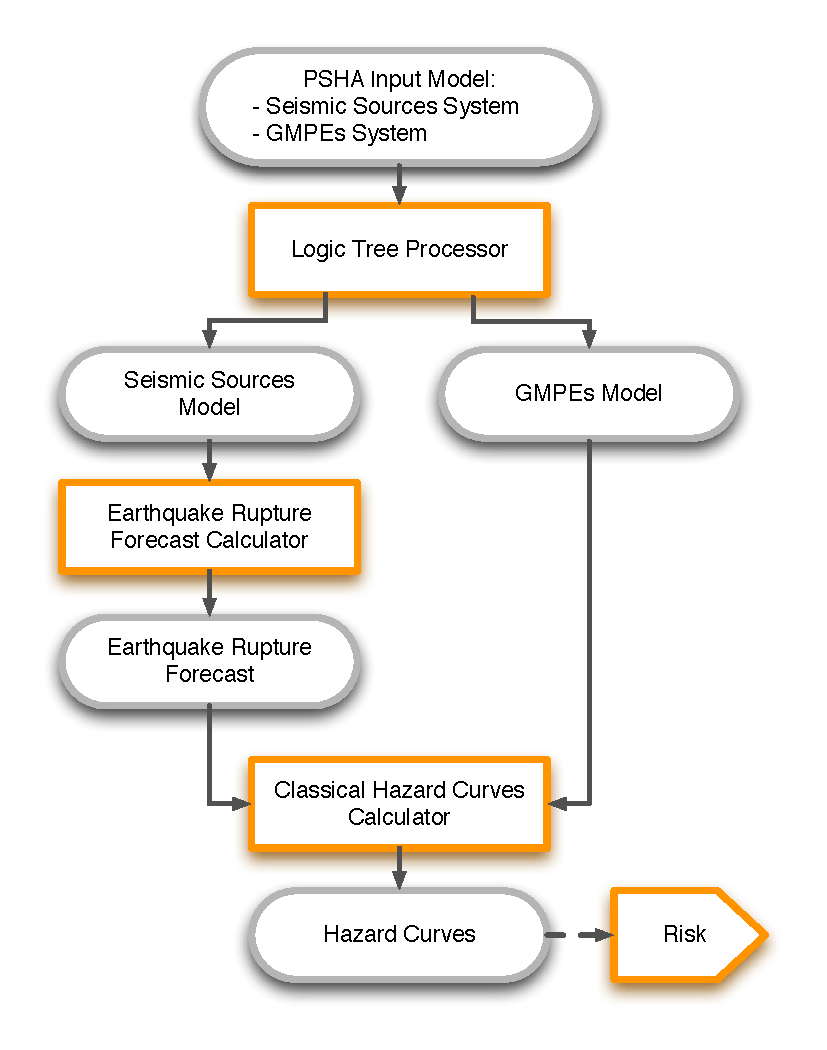
\includegraphics[width=12cm]{./Figures/Part_Hazard/classical_psha_workflow.eps}
\caption{Workflow for classical PSHA (boxes with purple border represent the 
calculators). Given a PSHA Input Model 
the Logic Tree Processor is responsible for creating a Seismic Sources model
and a ground motion model. 
The Seismic Sources model is then provided to the Earthquake Rupture Forecast 
calculator, which computes the ERF (the list of all earthquake ruptures in the 
source model with their probabilities of occurrence). 
Using the ERF and the GMPEs model the Classical PSHA calculator produces 
curves at the sites of interest.}
\label{classical_psha_workflow}
\end{center}
\end{figure}
% . . . . . . . . . . . . . . . . . . . . . . . . . . . . . . . . . . . < Figure
% ..............................................................................

As represented in Figure \ref{classical_psha_workflow}, the main calculators 
used to perform this analysis are:
\begin{enumerate}
%
\item \emph{Logic Tree Processor} \hfill \\
The Logic Tree Processor takes as an input the PSHA Input model. In case of 
the Seismic Sources, using the one of the Initial Seismic Sources Models and 
and by 'harvesting' the information contained in the Seismic Sources Logic Tree
- that is to sample the epistemic uncertainties - it creates a Seismic Sources 
Model (i.e. a model describing geometry and activity rates of each source 
without any epistemic uncertainty). 
%
Following the procedure just described the Logic Tree Processor creates a 
Ground Motion model (i.e. a data structure that associates to each tectonic 
region considered in the calculation a GMPE).
%
\item \emph{Earthquake Rupture Forecast Calculator} \hfill \\
The produced Seismic Sources Model is then used as input for the Earthquake 
Rupture Forecast (ERF) calculator which computes the probability of occurrence, 
over a specified time span, for each earthquake rupture produced by the source 
model.
\item \emph{Classical PSHA Calculator} \hfill \\
The cPSHA uses the ERF and the Ground Motion model to compute hazard curves on 
each site specified in the calculation settings.
\end{enumerate} 
%
%  - - - - - - - - - - - - - - - - - - - - - - - - - - - - - - - - - - - - - - -
\subsection{Event-Based Probabilistic Seismic Hazard Analysis}
\label{section:event-basedPSHA}
Input data for the Event-Based PSHA - as in the case of the Classical PSHA 
calculator - consist of a PSHA Input Model supplied to OQ together with a 
set of calculation settings.
%
% ..............................................................................
% . . . . . . . . . . . . . . . . . . . . . . . . . . . . . . . . . . . > Figure
\begin{figure}
\centering
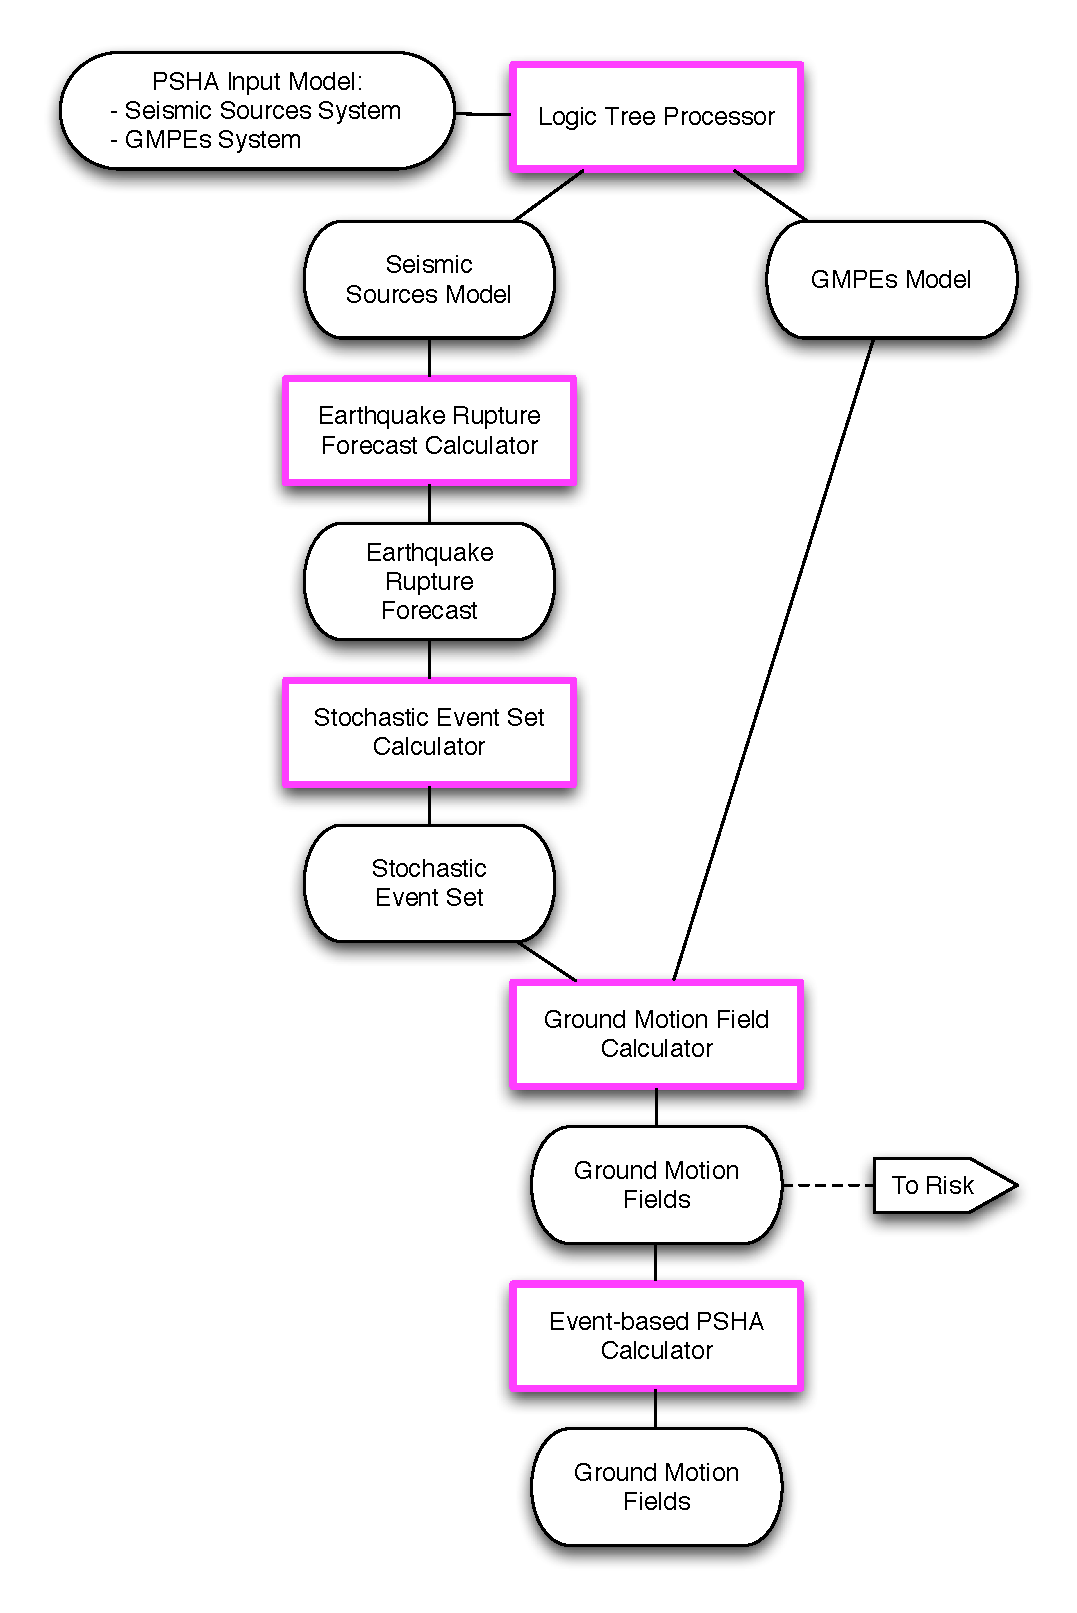
\includegraphics[width=12cm]{./Figures/Part_Hazard/event_based_workflow.eps}
\caption{Workflow for event-based PSHA. Similarly to the classical PSHA workflow 
(Figure \ref{classical_psha_workflow}), an ERF is computed, which is then used 
to generate a stochastic event set (representative of the seismic activity of 
a region in a given time span). Each event is then utilized to calculate a 
ground motion field over a region of interest.}
\label{event_based_workflow}
\end{figure}
% . . . . . . . . . . . . . . . . . . . . . . . . . . . . . . . . . . . < Figure
% ..............................................................................
As represented in Figure \ref{event_based_workflow}, the main calculators 
used to perform this analysis are:
\begin{enumerate}
%
\item \emph{Logic Tree Processor} \hfill \\
The Logic Tree Processor was already 
introduced in the description of the cPSHA workflow (see section 
\ref{section:classicalPSHA} at page \pageref{section:classicalPSHA}).
%
\item \emph{Earthquake Rupture Forecast Calculator} \hfill \\ 
The Logic Tree Processor was already 
introduced in the description of the cPSHA workflow (see section 
\ref{section:classicalPSHA} at page \pageref{section:classicalPSHA}).
%
\item \emph{Stochastic Event Set Calculator} \hfill \\
The Stochastic Event Set Calculator generates a Stochastic Event set 
by sampling each rupture contained in the ERF according to its 
probability of occurrence. Usually a Stochastic Event Set (SES) contains
a large number of seismicity history each one representative of a  
possible collection of events that can be produced by the seismic sources
considered in an analysis during the time span fixed for the calculation
of hazard (normally corresponding to 50 years).
%
\item \emph{Ground Motion Field Calculator} \hfill \\
The Ground Motion Field Calculator computes for each event contained in a 
Stochastic Event Set - provided as an input - a realization of the 
ground shaking taking into account the aleatory uncertainties in 
the ground motion model. Eventually, the Ground Motion Field calculator 
can consider the spatial correlation of the ground motion during the 
generation of the GMF.
%
\item \emph{Event-based PSHA Calculator} \hfill \\
The event-based PSHA calculator takes a (large) set of ground motion 
fields representative of the possible shaking that the investigated 
area can eventually experience over a (large) time span and for each 
grid node in a ground motion fields computes the corresponding hazard 
curve. 
%
This procedure is computationally intensive and is not recommended for 
investigating the hazard over large areas. 
\end{enumerate}

The Logic Tree Processor and the Earthquake rupture forecast were already 
introduced during the descrption of the cPSHA workflow (see section 
\ref{section:classicalPSHA} at page \pageref{section:classicalPSHA}).
%
%  - - - - - - - - - - - - - - - - - - - - - - - - - - - - - - - - - - - - - - -
\subsection{Deterministic Seismic Hazard Analysis}
\label{section:deterministicSHA}
% Deterministic
For deterministic SHA (DSHA), the input data consist of a single earthquake 
rupture model and a single ground motion model. Using the Ground Motion Field 
Calculator, multiple realizations of ground shaking can be computed, each 
realization sampling the aleatory uncertainties in the ground motion model.

As represented in Figure \ref{deterministic_workflow}, the main calculators 
used to perform this analysis are:
\begin{enumerate}
\item \emph{Ground Motion Field Calculator} \hfill \\
The Ground Motion Field Calculator was already 
introduced during the descrption of the ePSHA workflow (see section 
\ref{section:event-basedPSHA} at page \pageref{section:classicalPSHA}).
\end{enumerate}
% ..............................................................................
% . . . . . . . . . . . . . . . . . . . . . . . . . . . . . . . . . . . > Figure
\begin{figure}[!hb]
\centering
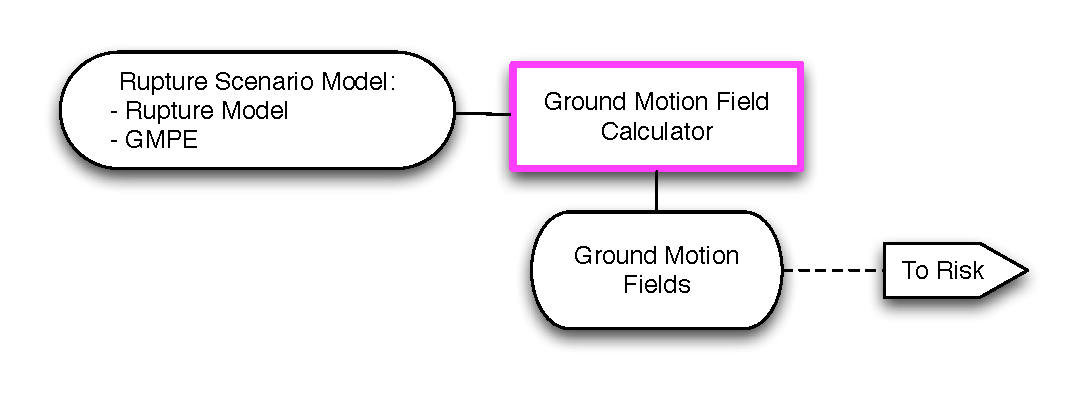
\includegraphics[width=12cm]{./Figures/Part_Hazard/deterministic_workflow.eps}
\caption{Workflow for deterministic SHA. Given a rupture scenario model, 
consisting of an earthquake rupture model, plus a GMPE, the ground motion 
field calculator can compute multiple ground motion field realizations (by 
taking into account GMPE aleatory uncertainties).}
\label{deterministic_workflow}
\end{figure}
% ..............................................................................
% . . . . . . . . . . . . . . . . . . . . . . . . . . . . . . . . . . . > Figure
%
% More details in the next chapters
%Next chapters discuss in more details the data model and the calculators. 
%Chapter \ref{chap:hazinp} describe the input data definition, that is the 
%different options for modeling seismogenic sources and how to include 
%epistemic uncertainties in both seismicity and ground motion models in 
%the form of a logic tree; Chapter \ref{chap:hazinp} also incorporates 
%the description of the logic tree structure adopted. 
%
%The methodology adopted to process the logic tree structure and the 
%definition and modeling of earthquake ruptures for the different 
%seismogenic source typologies are the topics of Chapter \ref{chap:erf}. 
%
%Chapter \ref{chap:hazcalc} describes the theoretical framework behind the main 
%hazard calculator available in OpenQuake: classical PSHA calculator and event 
%based calculator.
\chapter{Getting started}
	The present manual provides instructions about using OpenQuake to perform seismic hazard and risk analysis. However, no attempts are made to explain the "science" behind the software. The scientific basis and methodologies adopted in the software are illustrated in a separate document, the 'OpenQuake Book':\\
\href{http://openquake.org/wp-content/uploads/2011/10/OpenQuake-Book_Version0.1.pdf}
   {http://openquake.org/wp-content/uploads/2011/10/OpenQuake-Book-Version0.1.pdf}\\ \\
We refer the reader to the OpenQuake Book for a detailed explanation of the algorithms utilized, and indeed we strongly suggest its reading as a prerequisite for utilizing and understanding the present manual.

\section{Installing OpenQuake}
The OpenQuake installation is currently supported on the Ubuntu Operating System (\href{http://www.ubuntu.com/}
   {http://www.ubuntu.com/}), and installation instructions can be find here:\\ \\
    \href{https://github.com/gem/openquake/wiki/Ubuntu-11.04}
   {https://github.com/gem/openquake/wiki/Ubuntu-11.04}\\ \\
Installation on Mac OS X and Windows is not supported, however a workaround is possible by using a virtual machine. For instruction see here:\\ \\
\href{https://github.com/gem/openquake/wiki/Mac-OS-X}
   {https://github.com/gem/openquake/wiki/Mac-OS-X}   for Mac\\ \\
   and here:\\ \\
   \href{https://github.com/gem/openquake/wiki/Windows-OS}
   {https://github.com/gem/openquake/wiki/Windows-OS} for Windows.\\ \\
As an alternative of locally installing OpenQuake, the GEM-Model Facility has developed the OpenQuake Alpha Testing Service that gives the possibility to access the latest OpenQuake Alpha release on a cloud based server:\\ \\
\href{http://openquake.org/alpha-testing-services/}
   {http://openquake.org/alpha-testing-services/}

\section{OpenQuake Calculators and Input definition}
OpenQuake offers the possibility to perform different types of analysis/calculations for seismic hazard assessment:
\begin{itemize}
\item Classical (Cornell-type) PSHA
\item Event based PSHA
\item Disaggregation 
\item Uniform Hazard Spectra 
\item Deterministic (single earthquake scenario) SHA
\end{itemize}

and for seismic risk assessment:
\begin{itemize}
\item ...
\item ...
\end{itemize}

For each type of analysis, a configuration file (consisting of statements in the format \Verb+KEY=VALUE+) and one or more input data files in nrML format (an XML based format) are required.

The configuration file consists of three sections:
\begin{Verbatim}[frame=single, commandchars=\\\{\}, samepage=true]
[\textcolor{red}{general}]
...
[\textcolor{green}{HAZARD}]
...
[\textcolor{blue}{RISK}]
...
\end{Verbatim}
 
The \Verb+[general]+ section contains calculation parameters that are common to both hazard and risk analysis, while the \Verb+[HAZARD]+ and \Verb+[RISK]+ sections contains parameters specific for hazard and risk analysis, respectively.

The different types of analysis can be selected inside the \Verb+[general]+ section, by setting  the \Verb+CALCULATION_MODE+ key:
\begin{Verbatim}[frame=single, commandchars=\\\{\}, samepage=true]
[\textcolor{red}{general}]

CALCULATION_MODE =
\end{Verbatim}

Valid values are: 
\begin{itemize}
\item \Verb+Classical+ (for Classical PSHA)
\item \Verb+Event Based+ (for Event Based PSHA)
\item \Verb+Disaggregation+ (for Disaggregation analysis)
\item \Verb+UHS+ (for Uniform Hazard Spectra calculation)
\item \Verb+Deterministic+ ( for Deterministic SHA)
\item ...
\end{itemize}

Each analysis is performed over a set of geographical locations, that can be defined as grid points in a geographical region:

\begin{Verbatim}[frame=single, commandchars=\\\{\}, samepage=true]
[\textcolor{red}{general}]
...
REGION_VERTEX = LAT_1, LON_1, LAT_2, LON_2, ..., LAT_N, LON_N
REGION_GRID_SPACING = DELTA_GRID
\end{Verbatim}

where \Verb+REGION_VERTEX+ is a list of vertices coordinates (latitude, longitude) defining a polygonal region. The list of vertices can be defined in clock or counter-clock wise order. \Verb+REGION_GRID_SPACING+ defines the discretization step utilized for the grid construction. No restrictions are given in the number of vertices in the polygon definition.

A second option is to define a list of independent geographical locations:
\begin{Verbatim}[frame=single, commandchars=\\\{\}, samepage=true]
[\textcolor{red}{general}]
...
SITES = LAT_1, LON_1, LAT_2, LON_2,..., LAT_N, LON_N
\end{Verbatim}
each location being defined by latitude and longitude. Again no restrictions are given in the number of locations.

In case of risk analysis, a third option allows to perform calculations on the geographical locations defined in the exposure model. To select this option, the key \Verb+COMPUTE_HAZARD_AT_ASSETS_LOCATIONS+ must be set to \Verb+true+ in the \Verb+[RISK]+ section of the configuration file.
\begin{Verbatim}[frame=single, commandchars=\\\{\}, samepage=true]
[\textcolor{red}{RISK}]
...
COMPUTE_HAZARD_AT_ASSETS_LOCATIONS = true
\end{Verbatim}
if set to false, the region or sites defined in the \Verb+[general]+ section will be used instead.

Once the \Verb+CALCULATION_MODE+ and the locations of interest have been defined, the user is required to define the input data (in nrML format) and the calculation parameters (in the configuration file) for the requested analysis.

Chapters \ref{chap:hazinp} and \ref{chap:riskinp} describe the parameters and input data needed to perform all the supported hazard an risk analysis.
% ==============================================================================
% ------------------------------------------------------------------------- Part
\part{Hazard}
% ------------------------------------------------------------------------------
\chapter{Introduction}
	Probabilistic Seismic Hazard, a methodology largely 
founded on the works of \citet{cornell1968} and \citet{esteva1968}, 
nowadays contains a well established system of methods. 
%
The development of PSHA within the latest four decades did not change much of 
the original concept but made calculations more rigorous and accurate, 
especially with respect to the treatment of uncertainties. 

The evolution of PSHA methodologies proceeded in parallel with the development 
of instrumental seismology and hardware computing power. Computer codes such as
EQRISK \citep{mcguire1976} and the sequential versions of SEISRISK
\citep{bender1982,bender1987} traced the advancement of PSHA calculation within
the last part of the 20th century.

At the present time, the most computationally intensive PSHA models available 
are the ones developed for site-specific PSHA analyses, such as the ones 
performed for special installations or advanced regional PSHA input models 
(e.g. the UCERF2 model, \citet{field2009}) and the one used for large areas 
(e.g. continents or large nations) require powerful calculation facilities 
and sophisticated codes.
%
The computation demand posed by these model derives in the first case from 
the complexity of the input whilst in the second case is the number of sites 
that renders calculations particularly heavy.  

OpenQuake tries to cover this growing requirement for an accessible and 
efficient code for PSHA calculation. It's worth noting that the hazard 
component of OpenQuake leverages from OpenSHA (http://www.opensha.org) - 
an advanced, open-source, Java-based platform for conducting Seismic 
Hazard Analysis - and it is currently developed in collaboration with 
the OpenSHA team.  
%
% ------------------------------------------------------------------------------
\section{OpenQuake-hazard: main concepts}
Schematically, the procedure that OpenQuake follows to compute probabilistic 
seismic hazard is the following:
%
\begin{enumerate}
%
\item \emph{Read the PSHA input model - i.e. the union of the Seismic Sources 
System and the Ground Motion Model System - and calculation 
settings.}
	\index{Seismic Sources!System} %%%%%%
	\index{PSHA!Input model} %%%%%%
	\index{Ground Motion!Model!System} %%%%%%
	
	The \emph{Seismic Sources System} is an object that contains the 
	information necessary to create one or several Seismic Sources Model, 
	eventually by taking into account the epistemic uncertainties. 
	%
	The Seismic Sources System contains:
	\begin{itemize}
	\item One or several \emph{Initial Seismic Sources Models};
	\index{Logic Tree!Seismic sources} %%%%%%
	\item One logic tree - the Seismic Sources Logic Tree - describing 
	epistemic uncertainties connected with the objects and parameters 
	characterizing the Initial Seismic Sources Models.
	\end{itemize}
	
	The Ground Motion Model System is an object that contains the information 
	necessary to create (or use) one or several Ground Motion models, eventually 
	by taking into account the epistemic uncertainties. 
	\begin{itemize}
	\item One or several Ground Motion Models;
	\index{Logic Tree!Ground Motion Model} %%%%%%
	\item One logic tree - the Ground Motion Model Logic Tree - 
	describing epistemic uncertainties connected with the objects and 
	parameters characterizing the selected Ground Motion Models.	
	\end{itemize}

%
\item \emph{Process the logic tree structures to account for epistemic 
uncertainties connected with the seismic sources and the ground motion 
prediction equations and, create Seismic Sources Models and Ground Motion 
Prediction Equations Models}.
	\index{Seismic Sources!Model} %%%%%%
	\index{Ground Motion! Prediction Equations!Model} %%%%%%
	
	A Seismic Sources Model contains the information necessary to create an 
	Earthquake Rupture Forecast (i.e. the probabilistic seismicity occurrence
	model) without con\-sid\-er\-ing any epistemic uncertainty.
	%
	A Ground Motion Prediction E\-qua\-tions Model includes the information 
	necessary to compute hazard using a Seismic Sources Model. 
\item \emph{Compute the hazard considering as many Seismic Sources Models and 
Ground Motion Prediction Equations Models as need to adequately characterize 
uncertainties}.
\item \emph{Post-process the results obtained for distinct calculations}.
\end{enumerate}
%
% ------------------------------------------------------------------------------
\section{Calculation workflows}
% Three types of analysis
The hazard component of OpenQuake-Hazard performs seismic hazard 
analysis (SHA) following various approaches. 
%
Currently three main types of analysis are supported:
\begin{itemize}
\item \textit{Classical Probabilistic Seismic Hazard Analysis (cPSHA)}, 
allowing calculation of hazard curves and hazard maps following 
classical integration procedure 
(\cite{cornell1968}) as formulated by \cite{field2003}).
\item \textit{Event-Based Probabilistic Seismic Hazard Analysis (ePSHA)}, 
allowing calculation of ground motion fields from stochastic event sets.
\item \textit{Deterministic SHA (DSHA)}, allowing calculation of ground motion 
fields from single earthquake rupture scenario.
\end{itemize}
Each type of analysis has a modular structure, thus providing the capability 
of investigating all possible intermediate results. Moreover, each calculator 
can be expanded independently so that more calculation options/methodologies 
can be easily introduced, without affecting the overall calculation workflow.

Indeed each workflow described in the following Sections involves a number 
of calculators, each responsible for a specific task. 
Figures \ref{classical_psha_workflow}, \ref{event_based_workflow}, and 
\ref{deterministic_workflow} schematically depict the different calculation 
workflows.
%
%  - - - - - - - - - - - - - - - - - - - - - - - - - - - - - - - - - - - - - - -
\subsection{Classical Probabilistic Seismic Hazard Analysis}
\label{section:classicalPSHA}
%
Input data for the classical PSHA consist of a PSHA Input Model (PSHAim) that 
is provided together with a set of calculation settings. 
%
Chapter \ref{chap:hazinp} describes extensively the content of a PSHAim and 
in particular the different options for modeling seismogenic sources and the 
option offered to include epistemic uncertainties on both seismicity and 
ground motion models in the form of a logic tree; Chapter \ref{chap:hazinp} 
also incorporates the description of the logic tree structure adopted.
%
% ..............................................................................
% . . . . . . . . . . . . . . . . . . . . . . . . . . . . . . . . . . . > Figure
\begin{figure}[htbp]
\begin{center}
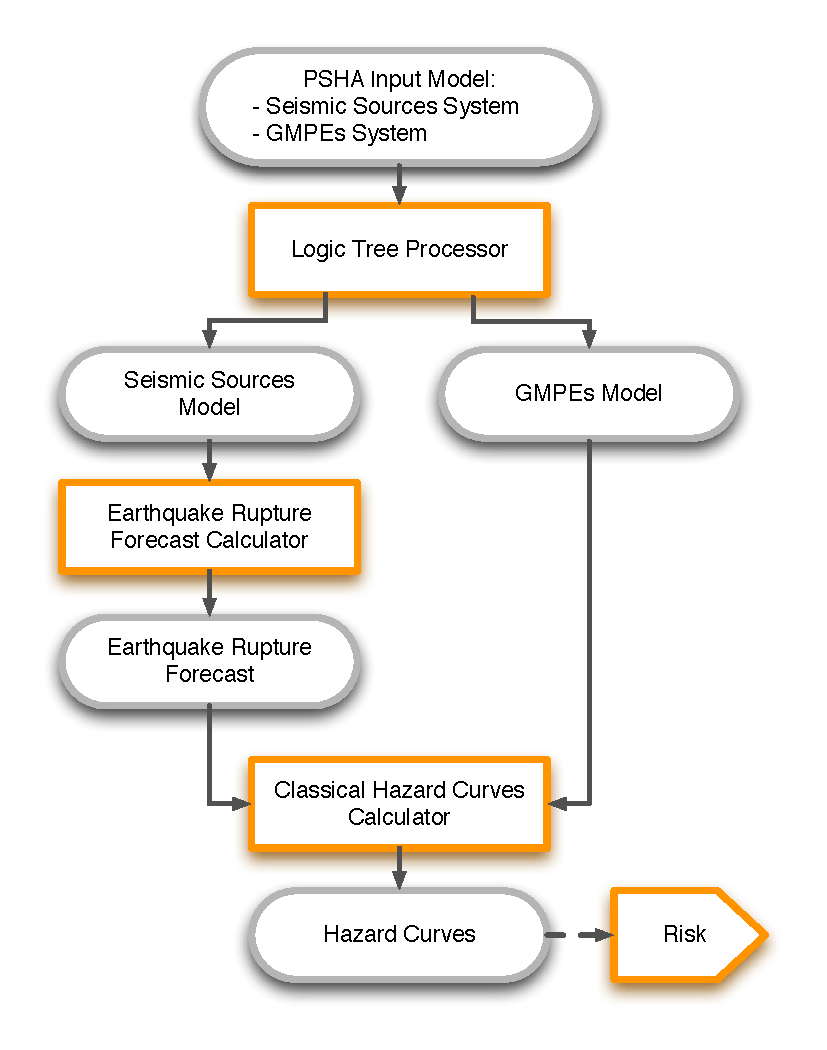
\includegraphics[width=12cm]{./Figures/Part_Hazard/classical_psha_workflow.eps}
\caption{Workflow for classical PSHA (boxes with purple border represent the 
calculators). Given a PSHA Input Model 
the Logic Tree Processor is responsible for creating a Seismic Sources model
and a ground motion model. 
The Seismic Sources model is then provided to the Earthquake Rupture Forecast 
calculator, which computes the ERF (the list of all earthquake ruptures in the 
source model with their probabilities of occurrence). 
Using the ERF and the GMPEs model the Classical PSHA calculator produces 
curves at the sites of interest.}
\label{classical_psha_workflow}
\end{center}
\end{figure}
% . . . . . . . . . . . . . . . . . . . . . . . . . . . . . . . . . . . < Figure
% ..............................................................................

As represented in Figure \ref{classical_psha_workflow}, the main calculators 
used to perform this analysis are:
\begin{enumerate}
%
\item \emph{Logic Tree Processor} \hfill \\
The Logic Tree Processor takes as an input the PSHA Input model. In case of 
the Seismic Sources, using the one of the Initial Seismic Sources Models and 
and by 'harvesting' the information contained in the Seismic Sources Logic Tree
- that is to sample the epistemic uncertainties - it creates a Seismic Sources 
Model (i.e. a model describing geometry and activity rates of each source 
without any epistemic uncertainty). 
%
Following the procedure just described the Logic Tree Processor creates a 
Ground Motion model (i.e. a data structure that associates to each tectonic 
region considered in the calculation a GMPE).
%
\item \emph{Earthquake Rupture Forecast Calculator} \hfill \\
The produced Seismic Sources Model is then used as input for the Earthquake 
Rupture Forecast (ERF) calculator which computes the probability of occurrence, 
over a specified time span, for each earthquake rupture produced by the source 
model.
\item \emph{Classical PSHA Calculator} \hfill \\
The cPSHA uses the ERF and the Ground Motion model to compute hazard curves on 
each site specified in the calculation settings.
\end{enumerate} 
%
%  - - - - - - - - - - - - - - - - - - - - - - - - - - - - - - - - - - - - - - -
\subsection{Event-Based Probabilistic Seismic Hazard Analysis}
\label{section:event-basedPSHA}
Input data for the Event-Based PSHA - as in the case of the Classical PSHA 
calculator - consist of a PSHA Input Model supplied to OQ together with a 
set of calculation settings.
%
% ..............................................................................
% . . . . . . . . . . . . . . . . . . . . . . . . . . . . . . . . . . . > Figure
\begin{figure}
\centering
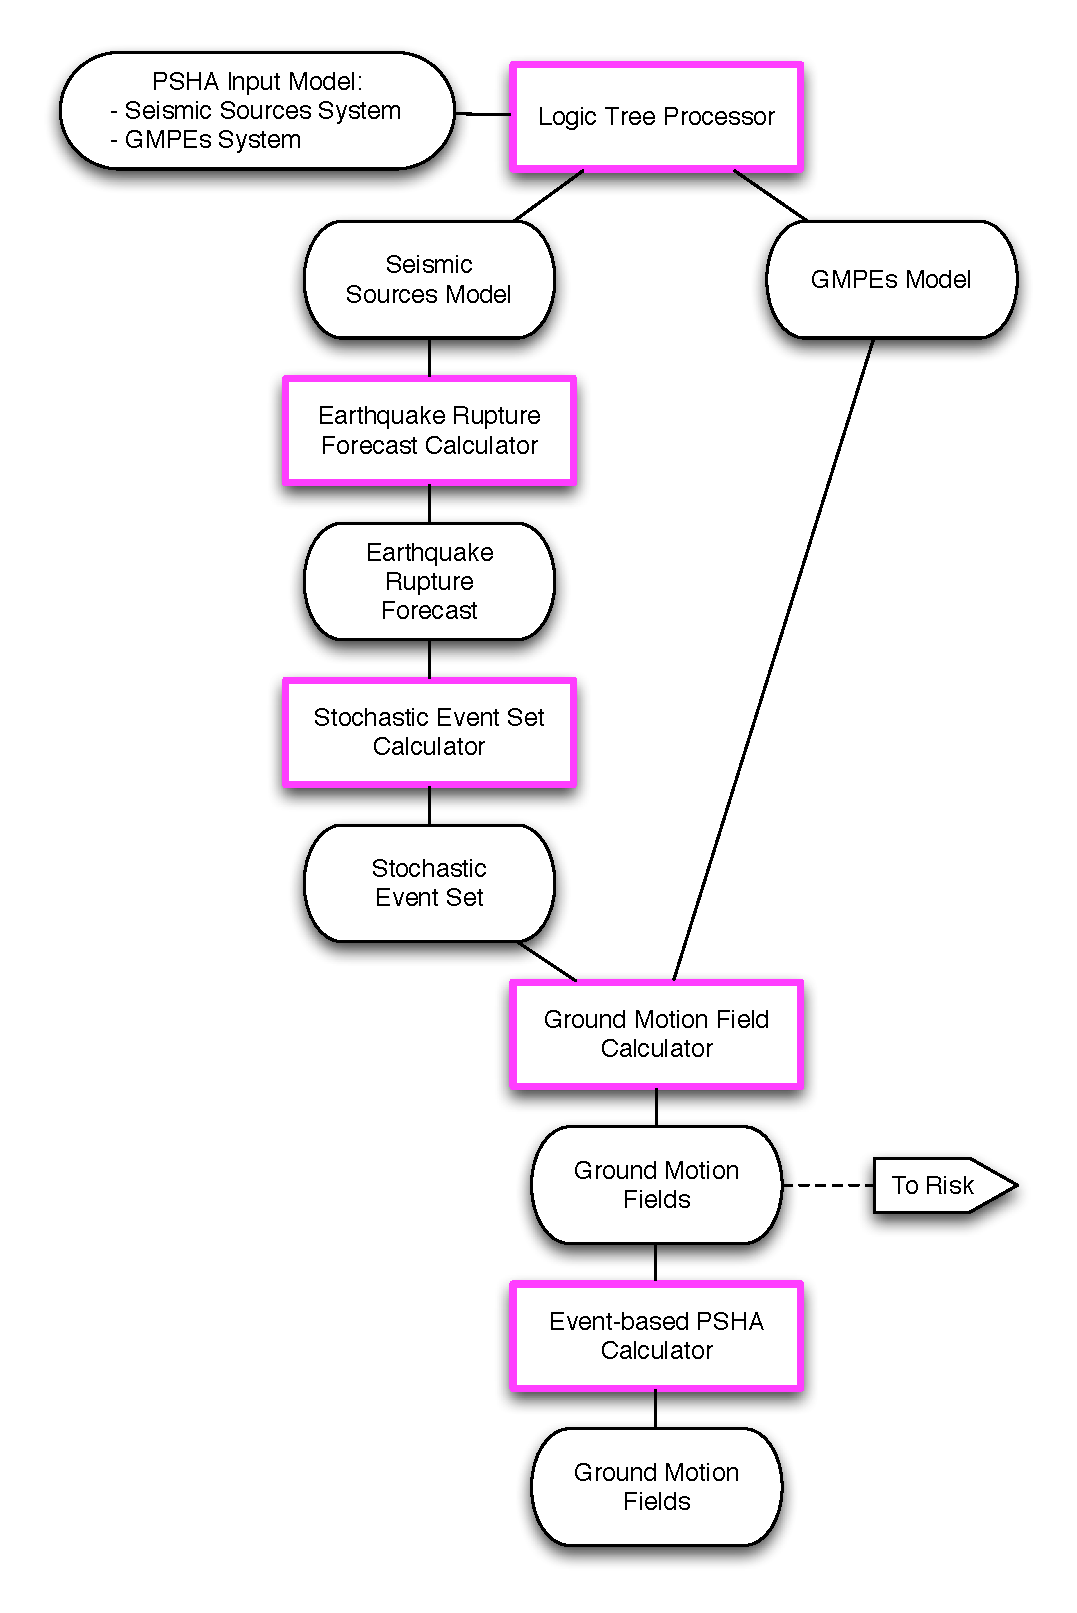
\includegraphics[width=12cm]{./Figures/Part_Hazard/event_based_workflow.eps}
\caption{Workflow for event-based PSHA. Similarly to the classical PSHA workflow 
(Figure \ref{classical_psha_workflow}), an ERF is computed, which is then used 
to generate a stochastic event set (representative of the seismic activity of 
a region in a given time span). Each event is then utilized to calculate a 
ground motion field over a region of interest.}
\label{event_based_workflow}
\end{figure}
% . . . . . . . . . . . . . . . . . . . . . . . . . . . . . . . . . . . < Figure
% ..............................................................................
As represented in Figure \ref{event_based_workflow}, the main calculators 
used to perform this analysis are:
\begin{enumerate}
%
\item \emph{Logic Tree Processor} \hfill \\
The Logic Tree Processor was already 
introduced in the description of the cPSHA workflow (see section 
\ref{section:classicalPSHA} at page \pageref{section:classicalPSHA}).
%
\item \emph{Earthquake Rupture Forecast Calculator} \hfill \\ 
The Logic Tree Processor was already 
introduced in the description of the cPSHA workflow (see section 
\ref{section:classicalPSHA} at page \pageref{section:classicalPSHA}).
%
\item \emph{Stochastic Event Set Calculator} \hfill \\
The Stochastic Event Set Calculator generates a Stochastic Event set 
by sampling each rupture contained in the ERF according to its 
probability of occurrence. Usually a Stochastic Event Set (SES) contains
a large number of seismicity history each one representative of a  
possible collection of events that can be produced by the seismic sources
considered in an analysis during the time span fixed for the calculation
of hazard (normally corresponding to 50 years).
%
\item \emph{Ground Motion Field Calculator} \hfill \\
The Ground Motion Field Calculator computes for each event contained in a 
Stochastic Event Set - provided as an input - a realization of the 
ground shaking taking into account the aleatory uncertainties in 
the ground motion model. Eventually, the Ground Motion Field calculator 
can consider the spatial correlation of the ground motion during the 
generation of the GMF.
%
\item \emph{Event-based PSHA Calculator} \hfill \\
The event-based PSHA calculator takes a (large) set of ground motion 
fields representative of the possible shaking that the investigated 
area can eventually experience over a (large) time span and for each 
grid node in a ground motion fields computes the corresponding hazard 
curve. 
%
This procedure is computationally intensive and is not recommended for 
investigating the hazard over large areas. 
\end{enumerate}

The Logic Tree Processor and the Earthquake rupture forecast were already 
introduced during the descrption of the cPSHA workflow (see section 
\ref{section:classicalPSHA} at page \pageref{section:classicalPSHA}).
%
%  - - - - - - - - - - - - - - - - - - - - - - - - - - - - - - - - - - - - - - -
\subsection{Deterministic Seismic Hazard Analysis}
\label{section:deterministicSHA}
% Deterministic
For deterministic SHA (DSHA), the input data consist of a single earthquake 
rupture model and a single ground motion model. Using the Ground Motion Field 
Calculator, multiple realizations of ground shaking can be computed, each 
realization sampling the aleatory uncertainties in the ground motion model.

As represented in Figure \ref{deterministic_workflow}, the main calculators 
used to perform this analysis are:
\begin{enumerate}
\item \emph{Ground Motion Field Calculator} \hfill \\
The Ground Motion Field Calculator was already 
introduced during the descrption of the ePSHA workflow (see section 
\ref{section:event-basedPSHA} at page \pageref{section:classicalPSHA}).
\end{enumerate}
% ..............................................................................
% . . . . . . . . . . . . . . . . . . . . . . . . . . . . . . . . . . . > Figure
\begin{figure}[!hb]
\centering
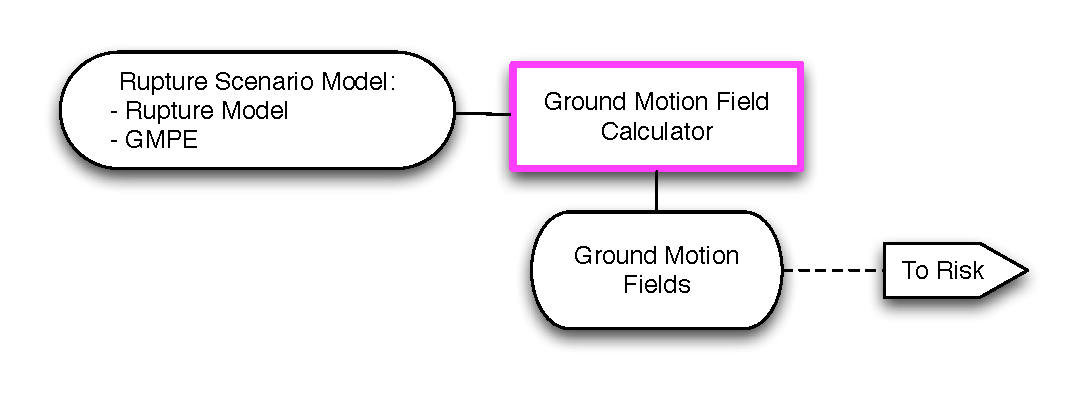
\includegraphics[width=12cm]{./Figures/Part_Hazard/deterministic_workflow.eps}
\caption{Workflow for deterministic SHA. Given a rupture scenario model, 
consisting of an earthquake rupture model, plus a GMPE, the ground motion 
field calculator can compute multiple ground motion field realizations (by 
taking into account GMPE aleatory uncertainties).}
\label{deterministic_workflow}
\end{figure}
% ..............................................................................
% . . . . . . . . . . . . . . . . . . . . . . . . . . . . . . . . . . . > Figure
%
% More details in the next chapters
%Next chapters discuss in more details the data model and the calculators. 
%Chapter \ref{chap:hazinp} describe the input data definition, that is the 
%different options for modeling seismogenic sources and how to include 
%epistemic uncertainties in both seismicity and ground motion models in 
%the form of a logic tree; Chapter \ref{chap:hazinp} also incorporates 
%the description of the logic tree structure adopted. 
%
%The methodology adopted to process the logic tree structure and the 
%definition and modeling of earthquake ruptures for the different 
%seismogenic source typologies are the topics of Chapter \ref{chap:erf}. 
%
%Chapter \ref{chap:hazcalc} describes the theoretical framework behind the main 
%hazard calculator available in OpenQuake: classical PSHA calculator and event 
%based calculator.
% ------------------------------------------------------------------------------
\chapter{OpenQuake hazard input description}
	\label{chap:hazinp}
	OpenQuake offers the possibility to perform different types of analysis/calculations for seismic hazard assessment:
\begin{itemize}
\item Classical (Cornell-type) PSHA
\item Event based PSHA
\item Disaggregation analysis
\item Uniform Hazard Spectra calculation
\item Deterministic (single earthquake scenario) SHA
\end{itemize}

and for seismic risk assessment:
\begin{itemize}
\item ...
\item ...
\end{itemize}

For each type of analysis, a configuration file (consisting of statements in the format \Verb+key=value+) and one or more input data files in nrML format (an XML based format) are required.

The different types of analysis can be selected inside the \Verb+[general]+ section of the configuration file, by setting  the \Verb+CALCULATION_MODE+ key:
\begin{Verbatim}[frame=single]
[general]

CALCULATION_MODE =
\end{Verbatim}

Valid values are: 
\begin{itemize}
\item \Verb+Classical+ (for Classical PSHA)
\item \Verb+Event Based+ (for Event Based PSHA)
\item \Verb+Disaggregation+ (for Disaggregation analysis)
\item \Verb+UHS+ (for Uniform Hazard Spectra calculation)
\item \Verb+Deterministic+ ( for Deterministic SHA)
\item ...
\end{itemize}

Each analysis is performed over a set of geographical locations, that can be defined as grid points in a geographical region:

\begin{Verbatim}[frame=single]
REGION_VERTEX = LAT_1, LON_1, LAT_2, LON_2, ..., LAT_N, LON_N
REGION_GRID_SPACING = DELTA_GRID
\end{Verbatim}

where \Verb+REGION_VERTEX+ is a list of vertices coordinates (latitude, longitude) defining a polygonal region. The list of vertices can be defined in clock or counter-clock wise order. \Verb+REGION_GRID_SPACING+ defines the discretization step utilized for the grid construction. No restrictions are given in the number of vertices in the polygon definition.

A second option is to define a list of independent geographical locations:
\begin{Verbatim}[frame=single]
SITES = LAT_1, LON_1, LAT_2, LON_2,..., LAT_N, LON_N
\end{Verbatim}
each location being defined by latitude and longitude. Again no restrictions are given in the number of locations.

In case of risk analysis, a third option allows to perform calculations on the geographical locations defined in the exposure model. To select this option, the key \Verb+COMPUTE_HAZARD_AT_ASSETS_LOCATIONS+ must be set to \Verb+true+ in the \Verb+[RISK]+ section of the configuration file.

Once the \Verb+CALCULATION_MODE+ and the locations of interest have been defined, the user is required to define the input data (in nrML format) and the calculation parameters (in the configuration file) for the requested analysis.

\section{Input Data definition for Classical, Event Based, Disaggregation and UHS}
Input data for probabilistic based seismic hazard analysis (Classical, Event based, Disaggregation, and UHS) are structured in terms of a:
\begin{itemize}
\item file describing the Seismic Source System, that is the set of initial source models and associated epistemic uncertainties needed to model the seismic activity in the region of interest.
\item file describing the Ground Motion System, that is the set of ground motion prediction equations, per tectonic region type, needed to model the ground motion shaking in the region of interest.
\end{itemize}
The paths to the Seismic Source and Ground Motion System files are given in the 
\Verb+SOURCE_MODEL_LOGIC_TREE_FILE+ and \Verb
+GMPE_LOGIC_TREE_FILE+ keys, respectively, both defined in the \Verb+[HAZARD]+ section of the configuration file.\\
The information required to define both the Seismic Source and Ground Motion Systems is stored in a \Verb+logicTree+ element: 
\begin{Verbatim}[frame=single, commandchars=\\\{\}]
<\textcolor{red}{logicTree} logicTreeID="ID">
...
</\textcolor{red}{logicTree}>
\end{Verbatim}
A \Verb+logicTree+ is defined as a sequence of \Verb+logicTreeBranchingLevel+ elements. The position in the sequence specifies in which level of the tree the branching level is located. That is, the first logicTreeBranchingLevel element in the sequence represents the first level in the tree, the second element the second level in the tree, and so on.
\begin{Verbatim}[frame=single, commandchars=\\\{\}]
<\textcolor{red}{logicTree} logicTreeID="ID">
	<\textcolor{green}{logicTreeBranchingLevel} branchingLevelID="ID_1">
		...
	</\textcolor{green}{logicTreeBranchingLevel}>
	<\textcolor{green}{logicTreeBranchingLevel} branchingLevelID="ID_2">
		...
	</\textcolor{green}{logicTreeBranchingLevel}>
	....
	<\textcolor{green}{logicTreeBranchingLevel} branchingLevelID="ID_N">
		...
	</\textcolor{green}{logicTreeBranchingLevel}>
</\textcolor{red}{logicTree}>
\end{Verbatim}
No restrictions are present on the number of tree levels that can be defined.\\
A \Verb+logicTreeBranchingLevel+ is defined as a sequence of \Verb+logicTreeBranchSet+ elements. Each \Verb+logicTreeBranchSet+ defines a particular epistemic uncertainty inside a branching level. A branch set has two required attributes (\Verb+branchingLevelID+ and \Verb+uncertaintyType+ (defining the type of epistemic uncertainty the branch set is defining))
\begin{Verbatim}[frame=single, commandchars=\\\{\}]
<\textcolor{red}{logicTree} logicTreeID="ID">
...
	<\textcolor{green}{logicTreeBranchingLevel} branchingLevelID="ID_#">
		<\textcolor{blue}{logicTreeBranchSet} branchSetID="ID_1"
			uncertaintyType="UNCERTAINTY_TYPE">
			...
		</\textcolor{blue}{logicTreeBranchSet}>
		<\textcolor{blue}{logicTreeBranchSet} branchSetID="ID_2"
			uncertaintyType="UNCERTAINTY_TYPE">
			...
		</\textcolor{blue}{logicTreeBranchSet}>
		...
		<\textcolor{blue}{logicTreeBranchSet} branchSetID="ID_N"
			uncertaintyType="UNCERTAINTY_TYPE">
			...
		</\textcolor{blue}{logicTreeBranchSet}>
	</\textcolor{green}{logicTreeBranchingLevel}>
...
</\textcolor{red}{logicTree}>
\end{Verbatim}
Possible values for the \Verb+uncertaintyType+ attribute are:
\begin{itemize}
\item \Verb+gmpeModel+: identifying epistemic uncertainties on ground motion prediction equations
\item \Verb+sourceModel+: identifying epistemic uncertainties on source models
\item \Verb+maxMagGRRelative+: identifying epistemic uncertainties (relative: that is increments) to be added (or subtracted, depending on the sign of the increment) to the Gutenberg-Richter maximum magnitude value.
\item \Verb+bGRRelative+: identifying epistemic uncertainties (relative) to be applied to the Gutenberg-Richter b value.
\item \Verb+abGRAbsolute+:identifying epistemic uncertainties (absolute: that is new values used to replace original values) on the Gutenberg-Richter a and b values.
\item \Verb+maxMagGRAbsolute+: identifying epistemic uncertainties (absolute) on the Gutenberg-Richter maximum magnitude.
\end{itemize}
No restrictions are given on the number of branch sets that can be defined inside a branching level.\\
A \Verb+branchSet+ is defined as a sequence of  \Verb+logicTreeBranch+ elements, each defined by an \Verb+uncertaintyModel+ element (a string identifying an uncertainty model; the content of the string varies with the uncertaintyType attribute value of the branchSet element) and the uncertaintyWeight element (specifying the probability/weight associated to the uncertaintyModel):
\begin{Verbatim}[frame=single, commandchars=\\\{\}]
<\textcolor{red}{logicTree} logicTreeID="ID">
...
	<\textcolor{green}{logicTreeBranchingLevel} branchingLevelID="ID_#">
		...
		<\textcolor{blue}{logicTreeBranchSet} branchSetID="ID_#"
				uncertaintyType="UNCERTAINTY_TYPE">
			<\textcolor{magenta}{logicTreeBranch} branchID="ID_1">
				<uncertaintyModel>
				UNCERTAINTY_MODEL
				</uncertaintyModel>
				<uncertaintyWeight>
				UNCERTAINTY_WEIGHT
				</uncertaintyWeight>
			</\textcolor{magenta}{logicTreeBranch}>
			...
			<\textcolor{magenta}{logicTreeBranch} branchID="ID_N">
				<uncertaintyModel>
				UNCERTAINTY_MODEL
				</uncertaintyModel>
				<uncertaintyWeight>
				UNCERTAINTY_WEIGHT
				</uncertaintyWeight>
			</\textcolor{magenta}{logicTreeBranch}>
		</\textcolor{blue}{logicTreeBranchSet}>
		...
	</\textcolor{green}{logicTreeBranchingLevel}>
...
</\textcolor{red}{logicTree}>
\end{Verbatim}
Depending on the \Verb+uncertaintyType+ the content of the \Verb+<uncertaintyModel>+ element changes:
\begin{itemize}
\item if \Verb+uncertaintyType="gmpeModel"+, the uncertainty model contains the name of a ground motion prediction equation (a list of available GMPEs are given in appendix A), e.g.:
\begin{Verbatim}[frame=single, commandchars=\\\{\}]
<uncertaintyModel>GMPE_NAME</uncertaintyModel>
\end{Verbatim}
\item if \Verb+uncertaintyType="sourceModel"+, the uncertainty model contains the paths to a source model file, e.g.:
\begin{Verbatim}[frame=single, commandchars=\\\{\}]
<uncertaintyModel>SOURCE_MODEL_FILE_PATH</uncertaintyModel>
\end{Verbatim}
\item if \Verb+uncertaintyType="maxMagGRRelative"+, the uncertainty model contains the increment to be added (or subtracted, depending on the sign) to the Gutenberg-Richter maximum magnitude:
\begin{Verbatim}[frame=single, commandchars=\\\{\}]
<uncertaintyModel>MAX_MAGNITUDE_INCREMENT</uncertaintyModel>
\end{Verbatim}
\item if \Verb+uncertaintyType="bGRRelative"+, the uncertainty model contains the increment to be added (or subtracted, depending on the sign) to the Gutenberg-Richter b value:
\begin{Verbatim}[frame=single, commandchars=\\\{\}]
<uncertaintyModel>B_VALUE_INCREMENT</uncertaintyModel>
\end{Verbatim}
\item if \Verb+uncertaintyType="abGRAbsolute"+, the uncertainty model contains one (if the uncertainty apply to a source with only one Gutenberg-Richter magnitude frequency distribution) or more (if the source has more than one magnitude frequency distributions) a and b pairs:
\begin{Verbatim}[frame=single, commandchars=\\\{\}]
<uncertaintyModel>
A_VALUE_1 B_VALUE_1
 ... 
A_VALUE_N B_VALUE_N
</uncertaintyModel>
\end{Verbatim}
\item if \Verb+uncertaintyType="maxMagGRAbsolute"+, the uncertainty model contains one or more (depending on the number of magnitude frequency distributions in the source) Gutenberg-Richter maximum magnitude values:
\begin{Verbatim}[frame=single, commandchars=\\\{\}]
<uncertaintyModel>
MAX_MAGNITUDE_1
 ... 
MAX_MAGNITUDE_N
</uncertaintyModel>
\end{Verbatim}
\end{itemize}
No restrictions are given on the number of \Verb+logicTreeBranch+ elements that can be defined in a \Verb+logicTreeBranchSet+, as long as the uncertainty weights sum to 1.0.\\
The \Verb+logicTreeBranchSet+ element offers also a number of optional attributes allowing for complex tree definitions:
\begin{itemize}
\item \Verb+applyToBranches+: specifies to which \Verb+logicTreeBranch+ elements (one or more), in the previous branching level, the branch set is linked to. The default is the keyword ALL, which means that a branch set is by default linked to all branches in the previous branching level. By specifying one or more branches to which the branch set links to, non-symmetric logic trees can be defined.
\item \Verb+applyToSources+: specifies to which source in a source model the uncertainty applies to.
\item \Verb+applyToSourceType+: specifies to which source type the uncertainty applies to.
\item \Verb+applyToTectonicRegionType+: specifies to which tectonic region type the uncertainty applies to.
\end{itemize}

\subsection{The Seismic Source System definition}
The Seismic Source System is defined in a \Verb+logicTreeElement+ with the following constrains:
\begin{itemize}
\item The first branching level can contain only one branch set. This branch set must define uncertainties in the source model (that is \Verb+uncertaintyType="sourceModel"+)
\item Subsequent branching levels can define uncertainties of type: \Verb+maxMagGRRelative+, \Verb+bGRRelative+, \Verb+abGRAbsolute+, \Verb+maxMagGRAbsolute+. Relative uncertainties are applied assuming conservation of total moment rate.
\item In all branching levels but the first, only one optional attribute (\Verb+applyToSources+, \Verb+applyToSourceType+, \Verb+applyToTectonicRegionType+) can be defined. The first branching level does not accept any optional attribute.
\item If in a branching level, a branch set has \Verb+applyToBranches="ALL"+, then this branch set must be unique in the branching level. In other words, only one branch set with \Verb+applyToBranches="ALL"+ is allowed per branching level.
\item If in a branching level, more than one branch sets are defined, the attribute \Verb+applyToBranches+ must contain one or more branch IDs referring to branches that are only in the previous branching level and that are not already linked to other branch sets (in other words there cannot be two branch sets that link to the same branch).
\item In all branch sets, branch weights must sum to 1.
\end{itemize}
Figure \ref{lt1} shows an example of Seismic Source System consisting of two initial source models defined in the first branching level. In the second branching level, absolute uncertainties on Gutenberg-Richter a and b values are defined for source model 1 (the  \Verb+applyToBranches="_11"). These uncertainties apply only to \Verb+area+ sources (applyToSourceType="area"). Same type of uncertainties are defined also for source model 2 (\Verb+applyToBranches="_12"+) but apply only to sources with IDs equal to \Verb+"_2"+ and \Verb+"_3"+ (\Verb+applyToSources="_2 _3"+). In the third branching level, absolute uncertainties on Gutenberg-Richter maximum magnitude are defined. These uncertainties apply to all source models in the previous branching level (the attribute \Verb+applyToBranches+ is absent, the default value \Verb+"ALL"+ is therefore assumed) but only to those sources that belongs to active shallow crust\\ (\Verb+applyToTectonicRegionType="Active Shallow Crust"+).
\begin{figure}[htbp]
\begin{center}
\begin{Verbatim}[frame=single, commandchars=\\\{\},fontsize=\scriptsize, samepage=true]
<\textcolor{red}{logicTree} logicTreeID="ID">
	<\textcolor{green}{logicTreeBranchingLevel} branchingLevelID="ID">
		<\textcolor{blue}{logicTreeBranchSet} branchSetID="ID"
		  uncertaintyType="\textcolor{orange}{sourceModel}">
			<\textcolor{magenta}{logicTreeBranch} branchID="_11">
			   <uncertaintyModel>SOURCE_MODEL_FILE_PATH</uncertaintyModel>
			   <uncertaintyWeight>WEIGHT</uncertaintyWeight>
			 </\textcolor{magenta}{logicTreeBranch}> 
			<\textcolor{magenta}{logicTreeBranch} branchID="_12">
			  <uncertaintyModel>SOURCE_MODEL_FILE_PATH</uncertaintyModel>
			  <uncertaintyWeight>WEIGHT</uncertaintyWeight>
			</\textcolor{magenta}{logicTreeBranch}>
		</\textcolor{blue}{logicTreeBranchSet}>
	</\textcolor{green}{logicTreeBranchingLevel}>
	<\textcolor{green}{logicTreeBranchingLevel} branchingLevelID="ID">
		<\textcolor{blue}{logicTreeBranchSet} branchSetID="ID" 
		    uncertaintyType="\textcolor{orange}{abGRAbsolute}"
		    applyToBranches="_11" 
		    applyToSourceType="area">
			<\textcolor{magenta}{logicTreeBranch} branchID="_11_12_21">
			   <uncertaintyModel>A_VALUE B_VALUE</uncertaintyModel>
			   <uncertaintyWeight>WEIGHT</uncertaintyWeight>
			</\textcolor{magenta}{logicTreeBranch}>
			<\textcolor{magenta}{logicTreeBranch} branchID="_11_12_22">
			   <uncertaintyModel>A_VALUE B_VALUE</uncertaintyModel>
			   <uncertaintyWeight>WEIGHT</uncertaintyWeight>
			</\textcolor{magenta}{logicTreeBranch}>  
		</\textcolor{blue}{logicTreeBranchSet}>
		<\textcolor{blue}{logicTreeBranchSet} branchSetID="ID" 
		   uncertaintyType="\textcolor{orange}{abGRAbsolute}"
	            applyToBranches="_12" 
		   applyToSources="_2 _3">
			<\textcolor{magenta}{logicTreeBranch} branchID="_13_21">
			   <uncertaintyModel>A_VALUE B_VALUE</uncertaintyModel>
			   <uncertaintyWeight>WEIGHT</uncertaintyWeight>
			   </\textcolor{magenta}{logicTreeBranch}>
			<\textcolor{magenta}{logicTreeBranch} branchID="_13_22">
			   <uncertaintyModel>A_VALUE B_VALUE</uncertaintyModel>
			   <uncertaintyWeight>WEIGHT</uncertaintyWeight>
			</\textcolor{magenta}{logicTreeBranch}>
		</\textcolor{blue}{logicTreeBranchSet}>
	</\textcolor{green}{logicTreeBranchingLevel}>
	<\textcolor{green}{logicTreeBranchingLevel} branchingLevelID="ID">
		<\textcolor{blue}{logicTreeBranchSet} branchSetID="ID" 
		   uncertaintyType="\textcolor{orange}{maxMagGRAbsolute}" 
		   applyToTectonicRegionType="Active Shallow Crust">
			<\textcolor{magenta}{logicTreeBranch} branchID="_31">
			   <uncertaintyModel>MAXIMUM_MAGNITUDE</uncertaintyModel>
			   <uncertaintyWeight>WEIGHT</uncertaintyWeight>
			</\textcolor{magenta}{logicTreeBranch}>
			<\textcolor{magenta}{logicTreeBranch} branchID="_32">
			   <uncertaintyModel>MAXIMUM_MAGNITUDE</uncertaintyModel>
			   <uncertaintyWeight>WEIGHT</uncertaintyWeight>
			</\textcolor{magenta}{logicTreeBranch}>
		</\textcolor{blue}{logicTreeBranchSet}>
	</\textcolor{green}{logicTreeBranchingLevel}>
</\textcolor{red}{logicTree}>
\end{Verbatim}
\caption{Example of Seismic Source System definition. Two source models are considered, and epistemic uncertainties (absolute) on Gutenberg-Richter a and b, and maximum magnitude are defined.}
\label{lt1}
\end{center}
\end{figure}
\subsection{The Ground Motion System definition}
The Ground Motion System is defined in a \Verb+logicTree+ element with the following constrains:
\begin{itemize}
\item Only one branch set can be defined per branching level.
\item Each branch set must define uncertainties of type \Verb+gmpeModel+.
\item All branch sets must define the applyToTectonicRegionType attribute. This is the only attribute allowed.
\item Each branch set must refer to a different tectonic region type.
\item In all branch sets, branch weights must sum to 1.
\end{itemize}
\begin{figure}[htbp]
\begin{center}
\begin{Verbatim}[frame=single, commandchars=\\\{\},fontsize=\scriptsize, samepage=true]
<\textcolor{red}{logicTree} logicTreeID="ID">       
	<\textcolor{green}{logicTreeBranchingLevel} branchingLevelID="ID">
		<\textcolor{blue}{logicTreeBranchSet} branchSetID="ID" uncertaintyType="gmpeModel" 
		applyToTectonicRegionType="\textcolor{orange}{Active Shallow Crust}">
			<\textcolor{magenta}{logicTreeBranch} branchID="ID">
				<uncertaintyModel>GMPE_NAME</uncertaintyModel>
				<uncertaintyWeight>WEIGHT</uncertaintyWeight>
			</\textcolor{magenta}{logicTreeBranch}>
			<\textcolor{magenta}{logicTreeBranch} branchID="ID">
				<uncertaintyModel>GMPE_NAME</uncertaintyModel>
				<uncertaintyWeight>WEIGHT</uncertaintyWeight>
			</\textcolor{magenta}{logicTreeBranch}>                
		</\textcolor{blue}{logicTreeBranchSet}>       
	</\textcolor{green}{logicTreeBranchingLevel}>
		<\textcolor{green}{logicTreeBranchingLevel} branchingLevelID="ID">
		<\textcolor{blue}{logicTreeBranchSet} branchSetID="ID" uncertaintyType="gmpeModel" 
		applyToTectonicRegionType="\textcolor{orange}{Stable Shallow Crust}">
			<\textcolor{magenta}{logicTreeBranch} branchID="ID">
				<uncertaintyModel>GMPE_NAME</uncertaintyModel>
				<uncertaintyWeight>WEIGHT</uncertaintyWeight>
			</\textcolor{magenta}{logicTreeBranch}>
			<\textcolor{magenta}{logicTreeBranch} branchID="ID">
				<uncertaintyModel>GMPE_NAME</uncertaintyModel>
				<uncertaintyWeight>WEIGHT</uncertaintyWeight>
			</\textcolor{magenta}{logicTreeBranch}>                
		</\textcolor{blue}{logicTreeBranchSet}>       
	</\textcolor{green}{logicTreeBranchingLevel}>
		<\textcolor{green}{logicTreeBranchingLevel} branchingLevelID="ID">
		<\textcolor{blue}{logicTreeBranchSet} branchSetID="ID" uncertaintyType="gmpeModel" 
		applyToTectonicRegionType="\textcolor{orange}{Subduction IntraSlab}">
			<\textcolor{magenta}{logicTreeBranch} branchID="ID">
				<uncertaintyModel>GMPE_NAME</uncertaintyModel>
				<uncertaintyWeight>WEIGHT</uncertaintyWeight>
			</\textcolor{magenta}{logicTreeBranch}>
			<\textcolor{magenta}{logicTreeBranch} branchID="ID">
				<uncertaintyModel>GMPE_NAME</uncertaintyModel>
				<uncertaintyWeight>WEIGHT</uncertaintyWeight>
			</\textcolor{magenta}{logicTreeBranch}>                
		</\textcolor{blue}{logicTreeBranchSet}>       
	</\textcolor{green}{logicTreeBranchingLevel}>
	<\textcolor{green}{logicTreeBranchingLevel} branchingLevelID="ID">
		<\textcolor{blue}{logicTreeBranchSet} branchSetID="ID" uncertaintyType="gmpeModel" 
		applyToTectonicRegionType="\textcolor{orange}{Subduction Interface}">
			<\textcolor{magenta}{logicTreeBranch} branchID="ID">
				<uncertaintyModel>GMPE_NAME</uncertaintyModel>
				<uncertaintyWeight>WEIGHT</uncertaintyWeight>
			</\textcolor{magenta}{logicTreeBranch}>                
		</\textcolor{blue}{logicTreeBranchSet}>
	</\textcolor{green}{logicTreeBranchingLevel}>
	<\textcolor{green}{logicTreeBranchingLevel} branchingLevelID="ID">
		<\textcolor{blue}{logicTreeBranchSet} branchSetID="ID" uncertaintyType="gmpeModel" 
		applyToTectonicRegionType="\textcolor{orange}{Volcanic}">
			<\textcolor{magenta}{logicTreeBranch} branchID="ID">
				<uncertaintyModel>GMPE_NAME</uncertaintyModel>
				<uncertaintyWeight>WEIGHT</uncertaintyWeight>
			</\textcolor{magenta}{logicTreeBranch}>                
		</\textcolor{blue}{logicTreeBranchSet}>
	</\textcolor{green}{logicTreeBranchingLevel}>           
</\textcolor{red}{logicTree}>
\end{Verbatim}
\caption{Example of Ground Motion System definition. GMPEs are defined for the tectonic region types currently supported by OpenQuake.}
\label{lt2}
\end{center}
\end{figure}

\subsection{Seismic source definition in nrML format}\label{seismicSourceNrml}
Four source typologies can be currently defined:
\begin{itemize}
\item Area
\item Point
\item Simple Fault
\item Complex Fault
\end{itemize}
Each source typology is identified by a specific element name in the nrML format:
\begin{itemize}
\item \Verb+areaSource+ (for Area)
\item \Verb+pointSource+ (for Point)
\item \Verb+simpleFaultSource+ (for Simple Fault)
\item \Verb+complexFaultSource+ (for Complex Fault)
\end{itemize}
and is characterized by three common attributes:
\begin{itemize}
\item ID: unique identifier 
\item name: source name
\item tectonic region type: tectonic region the source belongs to. 
\end{itemize}
The tectonic region type can be one of five typologies:
\begin{itemize}
\item \Verb+Active Shallow Crust+
\item \Verb+Stable Shallow Crust+
\item \Verb+Subduction Interface+
\item \Verb+Subduction IntraSlab+
\item \Verb+Volcanic+
\end{itemize}
In the nrML format, each source is therefore defined as follows:
\begin{itemize}
\item area:
\begin{Verbatim}[frame=single]
 <areaSource gml:id="SOURCE_ID">
    <gml:name>SOURCE_NAME</gml:name>
     <tectonicRegion>TECTONIC_REGION_TYPE</tectonicRegion>
      ...
\end{Verbatim}
\item point:
\begin{Verbatim}[frame=single]
<pointSource gml:id="SOURCE_ID">
    <gml:name>SOURCE_NAME</gml:name>
    <tectonicRegion>TECTONIC_REGION_TYPE</tectonicRegion>
     ...
\end{Verbatim}
\item simple fault:
\begin{Verbatim}[frame=single]
<simpleFaultSource gml:id="SOURCE_ID">
   <gml:name>SOURCE_NAME</gml:name>
   <tectonicRegion>TECTONIC_REGION_TYPE</tectonicRegion>
    ...
\end{Verbatim}
\item complex fault:
\begin{Verbatim}[frame=single]
<complexFaultSource gml:id="SOURCE_ID">
   <gml:name>SOURCE_NAME</gml:name>
   <tectonicRegion>TECTONIC_REGION_TYPE</tectonicRegion>
    ...
\end{Verbatim}
\end{itemize}
\subsubsection{Area source definition}
An area source can be utilized to describe a polygonal geographical region where seismicity is assumed to be uniform.
The geographic region is defined by the \Verb+areaBoundary+ element. More specifically the area boundary is defined by a list of vertices coordinates (longitude, latitude) in a \Verb+LinearRing+ element defining the exterior boundary of a \Verb+Polygon+ element:
\begin{Verbatim}[frame=single]
 <areaBoundary>
    <gml:Polygon>
      <gml:exterior>
        <gml:LinearRing>
           <gml:posList>
             LON_1 LAT_1
             LON_2 LAT_2
             ...			
             LON_N LAT_N
           </gml:posList>
         </gml:LinearRing>
        </gml:exterior>
      </gml:Polygon>
</areaBoundary>
\end{Verbatim}
The occurrence rates are specified in the \Verb+ruptureRateModel+ element, which contains the definition of a magnitude frequency distribution (\Verb+truncatedGutenbergRichter+ or \Verb+evenlyDiscretizedIncrementalMFD+) and a focal mechanism (\Verb+focalMechanism+).
\begin{Verbatim}[frame=single]
<ruptureRateModel>
   <truncatedGutenbergRichter> or <evenlyDiscretizedIncrementalMFD>
	...
   <focalMechanism>
	...
</ruptureRateModel>
\end{Verbatim}
A truncated Gutenberg-Richter magnitude frequency distribution is defined as follows:
\begin{Verbatim}[frame=single]
<truncatedGutenbergRichter>
   <aValueCumulative>CUMULATIVE_A_VALUE</aValueCumulative>
   <bValue>B_VALUE</bValue>
   <minMagnitude>MINIMUM_MAGNITUDE</minMagnitude>
   <maxMagnitude>MAXIMUM_MAGNITUDE</maxMagnitude>
</truncatedGutenbergRichter>
\end{Verbatim}
A generic evenly-discretized magnitude frequency distribution is defined instead as:
\begin{Verbatim}[frame=single]
<evenlyDiscretizedIncrementalMFD binSize="BIN_SIZE"
 	 minVal="MINIMUM_VALUE">
              RATE_1
              RATE_2
              ...
              RATE_N
</evenlyDiscretizedIncrementalMFD>
\end{Verbatim}
where \Verb+BIN_SIZE+ represents the discretization interval of the magnitude-frequency distribution, and \Verb+MINIMUM_VALUE+ represents the minimum value in the distribution (interpreted as the middle-point value of the first bin in the distribution).
A focal mechanism is defined in terms of a strike, dip and rake values:
\begin{Verbatim}[frame=single]
        <focalMechanism publicID="smi:fm1/0">
          <qml:nodalPlanes>
            <qml:nodalPlane1>
              <qml:strike>
                <qml:value>STRIKE_VALUE</qml:value>
              </qml:strike>
              <qml:dip>
                <qml:value>DIP_VALUE</qml:value>
              </qml:dip>
              <qml:rake>
                <qml:value>RAKE_VALUE</qml:value>
              </qml:rake>
            </qml:nodalPlane1>
          </qml:nodalPlanes>
        </focalMechanism>
 \end{Verbatim}
where $ 0^{\circ} \leq STRIKE_VALUE  \leq 360 ^{\circ}$
In a single area source definition, one or more \Verb+ruptureRateModel+ elements can be defined, so that multiple focal mechanisms (each having a specific magnitude-frequency distribution) can be defined:
\begin{Verbatim}[frame=single]
 <areaSource gml:id="SOURCE_ID">
 ...
 	<ruptureRateModel>
 	...
	 </ruptureRateModel>
	 <ruptureRateModel>
 	...
 	</ruptureRateModel>
...
 </areaSource>
\end{Verbatim}
\begin{comment}
\begin{Verbatim}[frame=single]
    <areaSource gml:id="src_1">
      <gml:name>Source 8.CH.3</gml:name>
      <tectonicRegion>Active Shallow Crust</tectonicRegion>
      <areaBoundary>
        <gml:Polygon>
          <gml:exterior>
            <gml:LinearRing>
              <gml:posList>-0.5 -0.5 -0.5 0.5 0.5 0.5 0.5 -0.5</gml:posList>
            </gml:LinearRing>
          </gml:exterior>
        </gml:Polygon>
      </areaBoundary>
      <ruptureRateModel>
        <truncatedGutenbergRichter>
          <aValueCumulative>2.5</aValueCumulative>
          <bValue>0.7318999871612379</bValue>
          <minMagnitude>5.0</minMagnitude>
          <maxMagnitude>8.0</maxMagnitude>
        </truncatedGutenbergRichter>
        <focalMechanism publicID="smi:fm1/0">
          <qml:nodalPlanes>
            <qml:nodalPlane1>
              <qml:strike>
                <qml:value>0.0</qml:value>
              </qml:strike>
              <qml:dip>
                <qml:value>90.0</qml:value>
              </qml:dip>
              <qml:rake>
                <qml:value>0.0</qml:value>
              </qml:rake>
            </qml:nodalPlane1>
          </qml:nodalPlanes>
        </focalMechanism>
      </ruptureRateModel>
      <ruptureDepthDistribution>
        <magnitude>6.5 7.5</magnitude>
        <depth>2.5 0.0</depth>
      </ruptureDepthDistribution>
      <hypocentralDepth>5.0</hypocentralDepth>
    </areaSource>
\end{Verbatim}
\end{comment}
\subsection{The Ground Motion System definition}
\begin{comment}
In this Chapter we provide with the reader a description of the input 
files containing the information necessary to completely describe a 
\gls{pshainputmodel} following a format compatible with \gls{acr:oq}. 
%
In OpenQuake the information commonly characterizing a 
\gls{pshainputmodel} is organized into - at least - four main files:
%
\begin{itemize}
	\item A \gls{configurationfile} (usually named config.gem) - It contains the 	
	\item A file describing the \gls{seismicsourcesystem}
	\item One or several files corresponding to the number of 
		\glspl{initialseismicsourcemodel}
	\item A file containing the information relative to the 
		\glspl{groundmotionsystem}
\end{itemize}

%
% ==============================================================================
\section{Anatomy of the configuration file for hazard calculation}
The configuration file contains the following parts
parts\footnote{
Each line starting with a cancel symbol is a comment line that is skipped
by the file parser.
}:
\begin{itemize}
	\item general 
	\item hazard
\end{itemize}
Each line starting with a cancel symbol is a comment line that is skipped
by the file parser. 

In order to discuss the content of the input file we use the 'config.gem' 
provided with the hazard demo relative to the PEER test set 1 case 10.

This is the general section of this file 
\begin{Verbatim}[baselinestretch=1,fontsize=\small,numbers=left,frame=single]
[general]
CALCULATION_MODE = Classical
# NOTE: The order of the vertices is to be kept!!!
# lat, lon of polygon vertices (in clock or counter-clock wise order)
REGION_VERTEX = 38.000, -122.000, 38.000, -122.000, 38.000, ...
# degrees
REGION_GRID_SPACING = 0.1
\end{Verbatim}
%
The first line contains a label specifying the section (in this 
particular case the 'general' section.

The second part composing the configuration file contains hazard 
specific information that can be divided into the following units: 
general calculation parameters and PSHA input model files, 
ground-motion model, seismic source model section and, results.
%
%
\subsubsection{General calculation parameters and PSHA input model files}
%
\begin{Verbatim}[baselinestretch=1,fontsize=\small,numbers=left,frame=single]
[HAZARD]
SOURCE_MODEL_LT_RANDOM_SEED = 23
GMPE_LT_RANDOM_SEED = 5
GMF_RANDOM_SEED = 3

# file containing erf logic tree structure
SOURCE_MODEL_LOGIC_TREE_FILE = source_model_logic_tree.xml
# file containing gmpe logic tree structure
GMPE_LOGIC_TREE_FILE = gmpe_logic_tree.xml
# output directory - relative to this file
OUTPUT_DIR = computed_output

# moment magnitude (Mw)
MINIMUM_MAGNITUDE = 5.0
# years
INVESTIGATION_TIME = 1.0
# maximum integration distance (km)
MAXIMUM_DISTANCE = 200.0
# bin width of the magnitude frequency distribution
WIDTH_OF_MFD_BIN = 0.1
\end{Verbatim}

%
% ============================================================================== 
\section{Description of the seismic source system file}
The seismic source system is described by an XML formatted file 
compatible with the NRML schema.
\marginpar{We miss a citation for NRML and a website as well!!}
%
\begin{Verbatim}[baselinestretch=1,fontsize=\small,numbers=left,frame=single]
	<logicTreeSet>
        <logicTree id="lt1">
            <logicTreeBranchSet branchingLevel="1" 
                                uncertaintyType="sourceModel">
                <logicTreeBranch>
                    <uncertaintyModel>source_model.xml</uncertaintyModel>
                    <uncertaintyWeight>1.0</uncertaintyWeight>
                </logicTreeBranch>
             </logicTreeBranchSet>
        </logicTree>
    </logicTreeSet>
\end{Verbatim}
%
% ------------------------------------------------------------------------------
\subsection{Basic seismic source typologies }

%
% ------------------------------------------------------------------------------
\subsection{Initial Seismic Source Model description}
The initial seismic source model used in this example is extremely simple, 
since it contains a single area source. 
%
\begin{Verbatim}[baselinestretch=1,fontsize=\small,numbers=left,frame=single]
    <areaSource gml:id="Src1">
      <gml:name>PEER test "AREA 1" model</gml:name>
      <tectonicRegion>Active Shallow Crust</tectonicRegion>
      <areaBoundary>
        <gml:Polygon>
          <gml:exterior>
            <gml:LinearRing>
              <gml:posList>
				-122.000 38.901 
				-121.920 38.899 
				...
				-122.160 38.892 
				-122.080 38.899 
			  </gml:posList>
            </gml:LinearRing>
          </gml:exterior>
        </gml:Polygon>
      </areaBoundary>
      <ruptureRateModel>
        <truncatedGutenbergRichter>
          <aValueCumulative>3.097</aValueCumulative>
          <bValue>0.9</bValue>
          <minMagnitude>5.0</minMagnitude>
          <maxMagnitude>6.5</maxMagnitude>
        </truncatedGutenbergRichter>
        <focalMechanism publicID="smi:f01/11">
          <qml:nodalPlanes>
            <qml:nodalPlane1>
              <qml:strike>
                <qml:value>0.0</qml:value>
              </qml:strike>
              <qml:dip>
                <qml:value>90.0</qml:value>
              </qml:dip>
              <qml:rake>
                <qml:value>0.0</qml:value>
              </qml:rake>
            </qml:nodalPlane1>
          </qml:nodalPlanes>
        </focalMechanism>
      </ruptureRateModel>
      <ruptureDepthDistribution>
        <magnitude>6.5</magnitude>
        <depth>5.0</depth>
      </ruptureDepthDistribution>
      <hypocentralDepth>5.0</hypocentralDepth>
    </areaSource>
  </sourceModel>
\end{Verbatim}


%
% ============================================================================== 
\section{Ground-motion system file description}
\end{comment}
% ------------------------------------------------------------------------------
\chapter{OpenQuake hazard calculation examples}
	\label{chap:hazexamples}
	\input{./oqum_Part_Hazard_Calc/calcExamples.tex}
% ==============================================================================
% ------------------------------------------------------------------------- Part
\part{Risk}
% ------------------------------------------------------------------------------
\chapter{Introduction}
	Probabilistic Seismic Hazard, a methodology largely 
founded on the works of \citet{cornell1968} and \citet{esteva1968}, 
nowadays contains a well established system of methods. 
%
The development of PSHA within the latest four decades did not change much of 
the original concept but made calculations more rigorous and accurate, 
especially with respect to the treatment of uncertainties. 

The evolution of PSHA methodologies proceeded in parallel with the development 
of instrumental seismology and hardware computing power. Computer codes such as
EQRISK \citep{mcguire1976} and the sequential versions of SEISRISK
\citep{bender1982,bender1987} traced the advancement of PSHA calculation within
the last part of the 20th century.

At the present time, the most computationally intensive PSHA models available 
are the ones developed for site-specific PSHA analyses, such as the ones 
performed for special installations or advanced regional PSHA input models 
(e.g. the UCERF2 model, \citet{field2009}) and the one used for large areas 
(e.g. continents or large nations) require powerful calculation facilities 
and sophisticated codes.
%
The computation demand posed by these model derives in the first case from 
the complexity of the input whilst in the second case is the number of sites 
that renders calculations particularly heavy.  

OpenQuake tries to cover this growing requirement for an accessible and 
efficient code for PSHA calculation. It's worth noting that the hazard 
component of OpenQuake leverages from OpenSHA (http://www.opensha.org) - 
an advanced, open-source, Java-based platform for conducting Seismic 
Hazard Analysis - and it is currently developed in collaboration with 
the OpenSHA team.  
%
% ------------------------------------------------------------------------------
\section{OpenQuake-hazard: main concepts}
Schematically, the procedure that OpenQuake follows to compute probabilistic 
seismic hazard is the following:
%
\begin{enumerate}
%
\item \emph{Read the PSHA input model - i.e. the union of the Seismic Sources 
System and the Ground Motion Model System - and calculation 
settings.}
	\index{Seismic Sources!System} %%%%%%
	\index{PSHA!Input model} %%%%%%
	\index{Ground Motion!Model!System} %%%%%%
	
	The \emph{Seismic Sources System} is an object that contains the 
	information necessary to create one or several Seismic Sources Model, 
	eventually by taking into account the epistemic uncertainties. 
	%
	The Seismic Sources System contains:
	\begin{itemize}
	\item One or several \emph{Initial Seismic Sources Models};
	\index{Logic Tree!Seismic sources} %%%%%%
	\item One logic tree - the Seismic Sources Logic Tree - describing 
	epistemic uncertainties connected with the objects and parameters 
	characterizing the Initial Seismic Sources Models.
	\end{itemize}
	
	The Ground Motion Model System is an object that contains the information 
	necessary to create (or use) one or several Ground Motion models, eventually 
	by taking into account the epistemic uncertainties. 
	\begin{itemize}
	\item One or several Ground Motion Models;
	\index{Logic Tree!Ground Motion Model} %%%%%%
	\item One logic tree - the Ground Motion Model Logic Tree - 
	describing epistemic uncertainties connected with the objects and 
	parameters characterizing the selected Ground Motion Models.	
	\end{itemize}

%
\item \emph{Process the logic tree structures to account for epistemic 
uncertainties connected with the seismic sources and the ground motion 
prediction equations and, create Seismic Sources Models and Ground Motion 
Prediction Equations Models}.
	\index{Seismic Sources!Model} %%%%%%
	\index{Ground Motion! Prediction Equations!Model} %%%%%%
	
	A Seismic Sources Model contains the information necessary to create an 
	Earthquake Rupture Forecast (i.e. the probabilistic seismicity occurrence
	model) without con\-sid\-er\-ing any epistemic uncertainty.
	%
	A Ground Motion Prediction E\-qua\-tions Model includes the information 
	necessary to compute hazard using a Seismic Sources Model. 
\item \emph{Compute the hazard considering as many Seismic Sources Models and 
Ground Motion Prediction Equations Models as need to adequately characterize 
uncertainties}.
\item \emph{Post-process the results obtained for distinct calculations}.
\end{enumerate}
%
% ------------------------------------------------------------------------------
\section{Calculation workflows}
% Three types of analysis
The hazard component of OpenQuake-Hazard performs seismic hazard 
analysis (SHA) following various approaches. 
%
Currently three main types of analysis are supported:
\begin{itemize}
\item \textit{Classical Probabilistic Seismic Hazard Analysis (cPSHA)}, 
allowing calculation of hazard curves and hazard maps following 
classical integration procedure 
(\cite{cornell1968}) as formulated by \cite{field2003}).
\item \textit{Event-Based Probabilistic Seismic Hazard Analysis (ePSHA)}, 
allowing calculation of ground motion fields from stochastic event sets.
\item \textit{Deterministic SHA (DSHA)}, allowing calculation of ground motion 
fields from single earthquake rupture scenario.
\end{itemize}
Each type of analysis has a modular structure, thus providing the capability 
of investigating all possible intermediate results. Moreover, each calculator 
can be expanded independently so that more calculation options/methodologies 
can be easily introduced, without affecting the overall calculation workflow.

Indeed each workflow described in the following Sections involves a number 
of calculators, each responsible for a specific task. 
Figures \ref{classical_psha_workflow}, \ref{event_based_workflow}, and 
\ref{deterministic_workflow} schematically depict the different calculation 
workflows.
%
%  - - - - - - - - - - - - - - - - - - - - - - - - - - - - - - - - - - - - - - -
\subsection{Classical Probabilistic Seismic Hazard Analysis}
\label{section:classicalPSHA}
%
Input data for the classical PSHA consist of a PSHA Input Model (PSHAim) that 
is provided together with a set of calculation settings. 
%
Chapter \ref{chap:hazinp} describes extensively the content of a PSHAim and 
in particular the different options for modeling seismogenic sources and the 
option offered to include epistemic uncertainties on both seismicity and 
ground motion models in the form of a logic tree; Chapter \ref{chap:hazinp} 
also incorporates the description of the logic tree structure adopted.
%
% ..............................................................................
% . . . . . . . . . . . . . . . . . . . . . . . . . . . . . . . . . . . > Figure
\begin{figure}[htbp]
\begin{center}
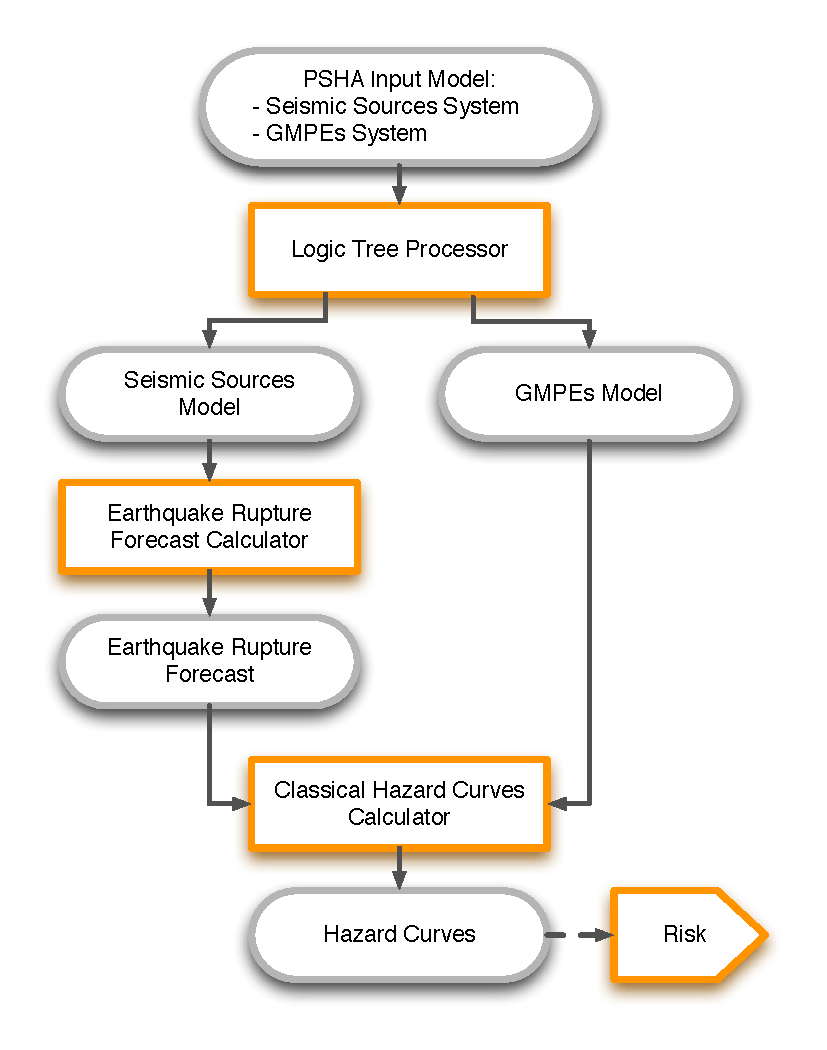
\includegraphics[width=12cm]{./Figures/Part_Hazard/classical_psha_workflow.eps}
\caption{Workflow for classical PSHA (boxes with purple border represent the 
calculators). Given a PSHA Input Model 
the Logic Tree Processor is responsible for creating a Seismic Sources model
and a ground motion model. 
The Seismic Sources model is then provided to the Earthquake Rupture Forecast 
calculator, which computes the ERF (the list of all earthquake ruptures in the 
source model with their probabilities of occurrence). 
Using the ERF and the GMPEs model the Classical PSHA calculator produces 
curves at the sites of interest.}
\label{classical_psha_workflow}
\end{center}
\end{figure}
% . . . . . . . . . . . . . . . . . . . . . . . . . . . . . . . . . . . < Figure
% ..............................................................................

As represented in Figure \ref{classical_psha_workflow}, the main calculators 
used to perform this analysis are:
\begin{enumerate}
%
\item \emph{Logic Tree Processor} \hfill \\
The Logic Tree Processor takes as an input the PSHA Input model. In case of 
the Seismic Sources, using the one of the Initial Seismic Sources Models and 
and by 'harvesting' the information contained in the Seismic Sources Logic Tree
- that is to sample the epistemic uncertainties - it creates a Seismic Sources 
Model (i.e. a model describing geometry and activity rates of each source 
without any epistemic uncertainty). 
%
Following the procedure just described the Logic Tree Processor creates a 
Ground Motion model (i.e. a data structure that associates to each tectonic 
region considered in the calculation a GMPE).
%
\item \emph{Earthquake Rupture Forecast Calculator} \hfill \\
The produced Seismic Sources Model is then used as input for the Earthquake 
Rupture Forecast (ERF) calculator which computes the probability of occurrence, 
over a specified time span, for each earthquake rupture produced by the source 
model.
\item \emph{Classical PSHA Calculator} \hfill \\
The cPSHA uses the ERF and the Ground Motion model to compute hazard curves on 
each site specified in the calculation settings.
\end{enumerate} 
%
%  - - - - - - - - - - - - - - - - - - - - - - - - - - - - - - - - - - - - - - -
\subsection{Event-Based Probabilistic Seismic Hazard Analysis}
\label{section:event-basedPSHA}
Input data for the Event-Based PSHA - as in the case of the Classical PSHA 
calculator - consist of a PSHA Input Model supplied to OQ together with a 
set of calculation settings.
%
% ..............................................................................
% . . . . . . . . . . . . . . . . . . . . . . . . . . . . . . . . . . . > Figure
\begin{figure}
\centering
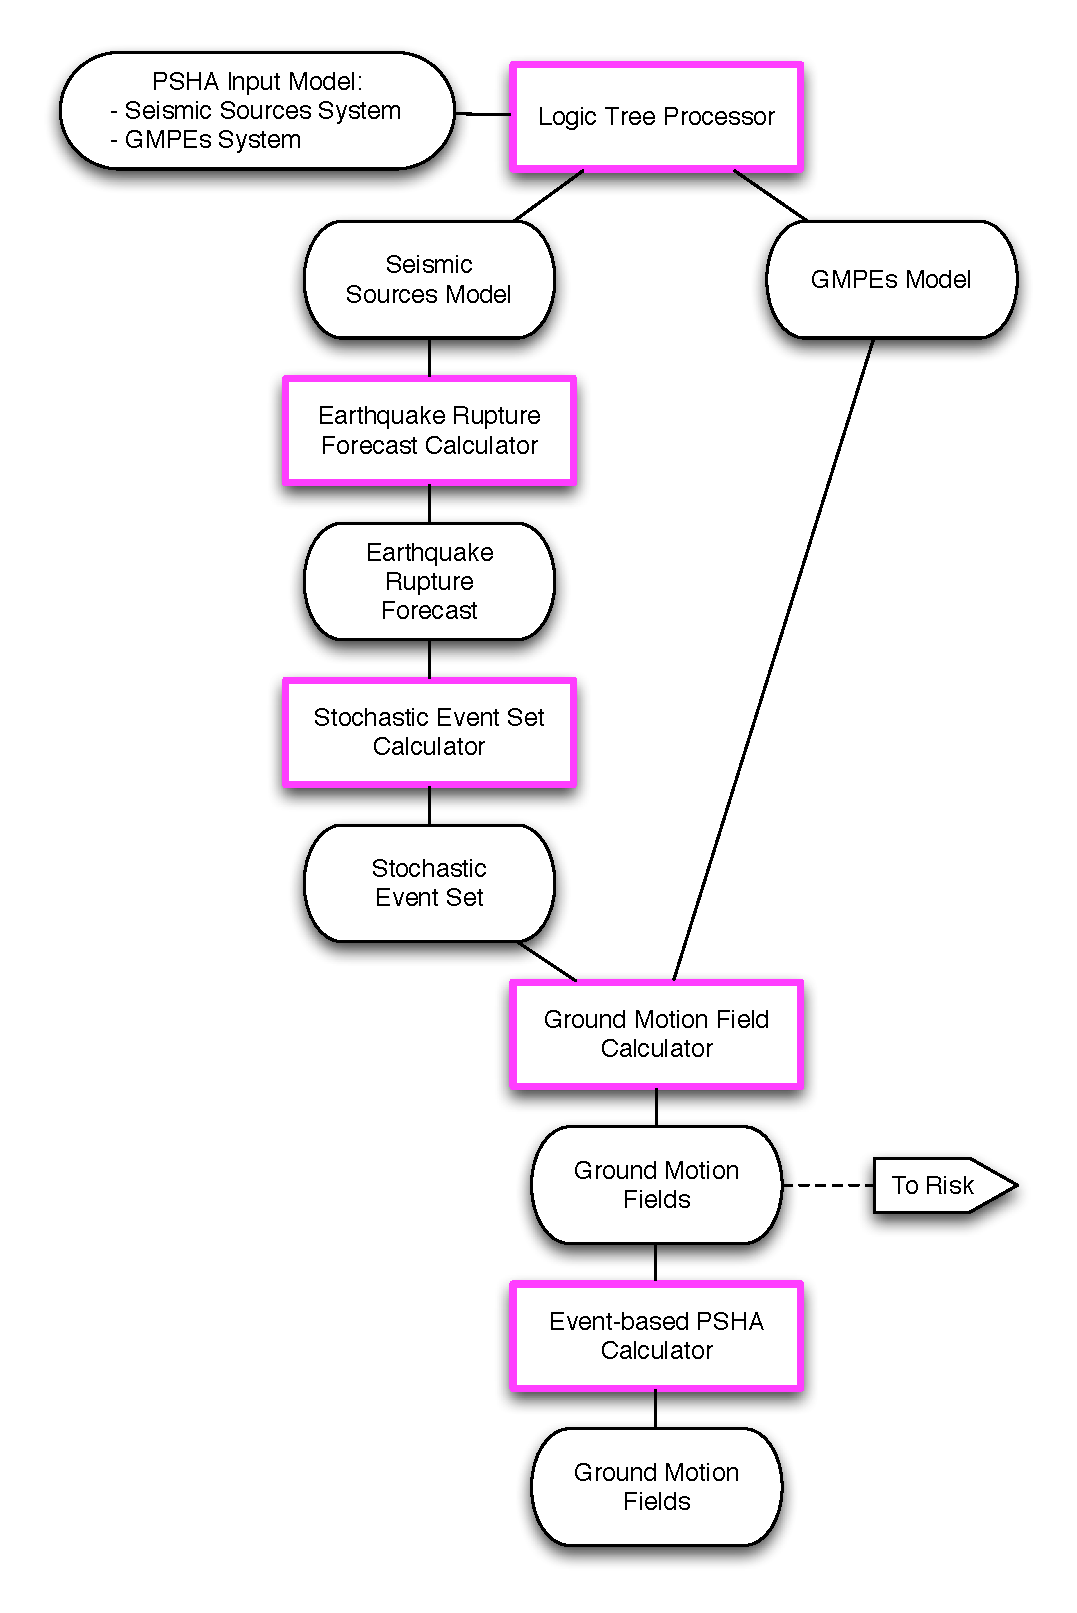
\includegraphics[width=12cm]{./Figures/Part_Hazard/event_based_workflow.eps}
\caption{Workflow for event-based PSHA. Similarly to the classical PSHA workflow 
(Figure \ref{classical_psha_workflow}), an ERF is computed, which is then used 
to generate a stochastic event set (representative of the seismic activity of 
a region in a given time span). Each event is then utilized to calculate a 
ground motion field over a region of interest.}
\label{event_based_workflow}
\end{figure}
% . . . . . . . . . . . . . . . . . . . . . . . . . . . . . . . . . . . < Figure
% ..............................................................................
As represented in Figure \ref{event_based_workflow}, the main calculators 
used to perform this analysis are:
\begin{enumerate}
%
\item \emph{Logic Tree Processor} \hfill \\
The Logic Tree Processor was already 
introduced in the description of the cPSHA workflow (see section 
\ref{section:classicalPSHA} at page \pageref{section:classicalPSHA}).
%
\item \emph{Earthquake Rupture Forecast Calculator} \hfill \\ 
The Logic Tree Processor was already 
introduced in the description of the cPSHA workflow (see section 
\ref{section:classicalPSHA} at page \pageref{section:classicalPSHA}).
%
\item \emph{Stochastic Event Set Calculator} \hfill \\
The Stochastic Event Set Calculator generates a Stochastic Event set 
by sampling each rupture contained in the ERF according to its 
probability of occurrence. Usually a Stochastic Event Set (SES) contains
a large number of seismicity history each one representative of a  
possible collection of events that can be produced by the seismic sources
considered in an analysis during the time span fixed for the calculation
of hazard (normally corresponding to 50 years).
%
\item \emph{Ground Motion Field Calculator} \hfill \\
The Ground Motion Field Calculator computes for each event contained in a 
Stochastic Event Set - provided as an input - a realization of the 
ground shaking taking into account the aleatory uncertainties in 
the ground motion model. Eventually, the Ground Motion Field calculator 
can consider the spatial correlation of the ground motion during the 
generation of the GMF.
%
\item \emph{Event-based PSHA Calculator} \hfill \\
The event-based PSHA calculator takes a (large) set of ground motion 
fields representative of the possible shaking that the investigated 
area can eventually experience over a (large) time span and for each 
grid node in a ground motion fields computes the corresponding hazard 
curve. 
%
This procedure is computationally intensive and is not recommended for 
investigating the hazard over large areas. 
\end{enumerate}

The Logic Tree Processor and the Earthquake rupture forecast were already 
introduced during the descrption of the cPSHA workflow (see section 
\ref{section:classicalPSHA} at page \pageref{section:classicalPSHA}).
%
%  - - - - - - - - - - - - - - - - - - - - - - - - - - - - - - - - - - - - - - -
\subsection{Deterministic Seismic Hazard Analysis}
\label{section:deterministicSHA}
% Deterministic
For deterministic SHA (DSHA), the input data consist of a single earthquake 
rupture model and a single ground motion model. Using the Ground Motion Field 
Calculator, multiple realizations of ground shaking can be computed, each 
realization sampling the aleatory uncertainties in the ground motion model.

As represented in Figure \ref{deterministic_workflow}, the main calculators 
used to perform this analysis are:
\begin{enumerate}
\item \emph{Ground Motion Field Calculator} \hfill \\
The Ground Motion Field Calculator was already 
introduced during the descrption of the ePSHA workflow (see section 
\ref{section:event-basedPSHA} at page \pageref{section:classicalPSHA}).
\end{enumerate}
% ..............................................................................
% . . . . . . . . . . . . . . . . . . . . . . . . . . . . . . . . . . . > Figure
\begin{figure}[!hb]
\centering
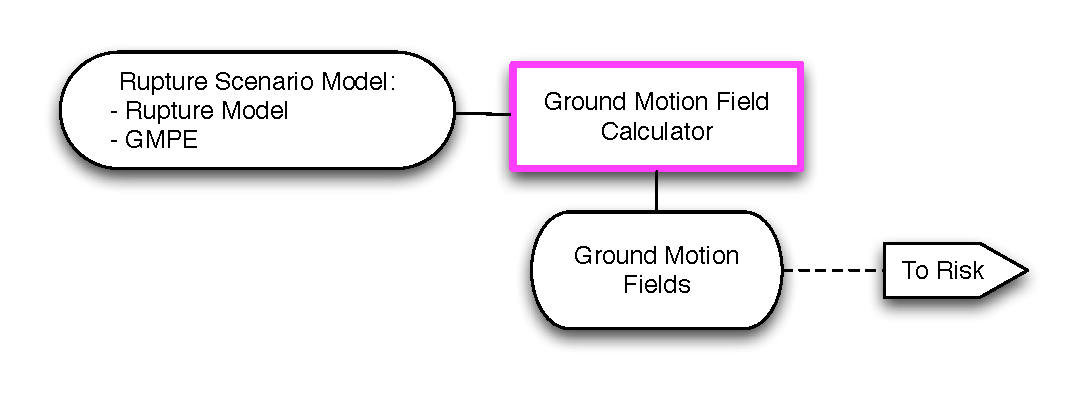
\includegraphics[width=12cm]{./Figures/Part_Hazard/deterministic_workflow.eps}
\caption{Workflow for deterministic SHA. Given a rupture scenario model, 
consisting of an earthquake rupture model, plus a GMPE, the ground motion 
field calculator can compute multiple ground motion field realizations (by 
taking into account GMPE aleatory uncertainties).}
\label{deterministic_workflow}
\end{figure}
% ..............................................................................
% . . . . . . . . . . . . . . . . . . . . . . . . . . . . . . . . . . . > Figure
%
% More details in the next chapters
%Next chapters discuss in more details the data model and the calculators. 
%Chapter \ref{chap:hazinp} describe the input data definition, that is the 
%different options for modeling seismogenic sources and how to include 
%epistemic uncertainties in both seismicity and ground motion models in 
%the form of a logic tree; Chapter \ref{chap:hazinp} also incorporates 
%the description of the logic tree structure adopted. 
%
%The methodology adopted to process the logic tree structure and the 
%definition and modeling of earthquake ruptures for the different 
%seismogenic source typologies are the topics of Chapter \ref{chap:erf}. 
%
%Chapter \ref{chap:hazcalc} describes the theoretical framework behind the main 
%hazard calculator available in OpenQuake: classical PSHA calculator and event 
%based calculator.
% ------------------------------------------------------------------------------
\chapter{OpenQuake input description}
	\label{chap:riskinp}
	OpenQuake offers the possibility to perform different types of analysis/calculations for seismic hazard assessment:
\begin{itemize}
\item Classical (Cornell-type) PSHA
\item Event based PSHA
\item Disaggregation analysis
\item Uniform Hazard Spectra calculation
\item Deterministic (single earthquake scenario) SHA
\end{itemize}

and for seismic risk assessment:
\begin{itemize}
\item ...
\item ...
\end{itemize}

For each type of analysis, a configuration file (consisting of statements in the format \Verb+key=value+) and one or more input data files in nrML format (an XML based format) are required.

The different types of analysis can be selected inside the \Verb+[general]+ section of the configuration file, by setting  the \Verb+CALCULATION_MODE+ key:
\begin{Verbatim}[frame=single]
[general]

CALCULATION_MODE =
\end{Verbatim}

Valid values are: 
\begin{itemize}
\item \Verb+Classical+ (for Classical PSHA)
\item \Verb+Event Based+ (for Event Based PSHA)
\item \Verb+Disaggregation+ (for Disaggregation analysis)
\item \Verb+UHS+ (for Uniform Hazard Spectra calculation)
\item \Verb+Deterministic+ ( for Deterministic SHA)
\item ...
\end{itemize}

Each analysis is performed over a set of geographical locations, that can be defined as grid points in a geographical region:

\begin{Verbatim}[frame=single]
REGION_VERTEX = LAT_1, LON_1, LAT_2, LON_2, ..., LAT_N, LON_N
REGION_GRID_SPACING = DELTA_GRID
\end{Verbatim}

where \Verb+REGION_VERTEX+ is a list of vertices coordinates (latitude, longitude) defining a polygonal region. The list of vertices can be defined in clock or counter-clock wise order. \Verb+REGION_GRID_SPACING+ defines the discretization step utilized for the grid construction. No restrictions are given in the number of vertices in the polygon definition.

A second option is to define a list of independent geographical locations:
\begin{Verbatim}[frame=single]
SITES = LAT_1, LON_1, LAT_2, LON_2,..., LAT_N, LON_N
\end{Verbatim}
each location being defined by latitude and longitude. Again no restrictions are given in the number of locations.

In case of risk analysis, a third option allows to perform calculations on the geographical locations defined in the exposure model. To select this option, the key \Verb+COMPUTE_HAZARD_AT_ASSETS_LOCATIONS+ must be set to \Verb+true+ in the \Verb+[RISK]+ section of the configuration file.

Once the \Verb+CALCULATION_MODE+ and the locations of interest have been defined, the user is required to define the input data (in nrML format) and the calculation parameters (in the configuration file) for the requested analysis.

\section{Input Data definition for Classical, Event Based, Disaggregation and UHS}
Input data for probabilistic based seismic hazard analysis (Classical, Event based, Disaggregation, and UHS) are structured in terms of a:
\begin{itemize}
\item file describing the Seismic Source System, that is the set of initial source models and associated epistemic uncertainties needed to model the seismic activity in the region of interest.
\item file describing the Ground Motion System, that is the set of ground motion prediction equations, per tectonic region type, needed to model the ground motion shaking in the region of interest.
\end{itemize}
The paths to the Seismic Source and Ground Motion System files are given in the 
\Verb+SOURCE_MODEL_LOGIC_TREE_FILE+ and \Verb
+GMPE_LOGIC_TREE_FILE+ keys, respectively, both defined in the \Verb+[HAZARD]+ section of the configuration file.\\
The information required to define both the Seismic Source and Ground Motion Systems is stored in a \Verb+logicTree+ element: 
\begin{Verbatim}[frame=single, commandchars=\\\{\}]
<\textcolor{red}{logicTree} logicTreeID="ID">
...
</\textcolor{red}{logicTree}>
\end{Verbatim}
A \Verb+logicTree+ is defined as a sequence of \Verb+logicTreeBranchingLevel+ elements. The position in the sequence specifies in which level of the tree the branching level is located. That is, the first logicTreeBranchingLevel element in the sequence represents the first level in the tree, the second element the second level in the tree, and so on.
\begin{Verbatim}[frame=single, commandchars=\\\{\}]
<\textcolor{red}{logicTree} logicTreeID="ID">
	<\textcolor{green}{logicTreeBranchingLevel} branchingLevelID="ID_1">
		...
	</\textcolor{green}{logicTreeBranchingLevel}>
	<\textcolor{green}{logicTreeBranchingLevel} branchingLevelID="ID_2">
		...
	</\textcolor{green}{logicTreeBranchingLevel}>
	....
	<\textcolor{green}{logicTreeBranchingLevel} branchingLevelID="ID_N">
		...
	</\textcolor{green}{logicTreeBranchingLevel}>
</\textcolor{red}{logicTree}>
\end{Verbatim}
No restrictions are present on the number of tree levels that can be defined.\\
A \Verb+logicTreeBranchingLevel+ is defined as a sequence of \Verb+logicTreeBranchSet+ elements. Each \Verb+logicTreeBranchSet+ defines a particular epistemic uncertainty inside a branching level. A branch set has two required attributes (\Verb+branchingLevelID+ and \Verb+uncertaintyType+ (defining the type of epistemic uncertainty the branch set is defining))
\begin{Verbatim}[frame=single, commandchars=\\\{\}]
<\textcolor{red}{logicTree} logicTreeID="ID">
...
	<\textcolor{green}{logicTreeBranchingLevel} branchingLevelID="ID_#">
		<\textcolor{blue}{logicTreeBranchSet} branchSetID="ID_1"
			uncertaintyType="UNCERTAINTY_TYPE">
			...
		</\textcolor{blue}{logicTreeBranchSet}>
		<\textcolor{blue}{logicTreeBranchSet} branchSetID="ID_2"
			uncertaintyType="UNCERTAINTY_TYPE">
			...
		</\textcolor{blue}{logicTreeBranchSet}>
		...
		<\textcolor{blue}{logicTreeBranchSet} branchSetID="ID_N"
			uncertaintyType="UNCERTAINTY_TYPE">
			...
		</\textcolor{blue}{logicTreeBranchSet}>
	</\textcolor{green}{logicTreeBranchingLevel}>
...
</\textcolor{red}{logicTree}>
\end{Verbatim}
Possible values for the \Verb+uncertaintyType+ attribute are:
\begin{itemize}
\item \Verb+gmpeModel+: identifying epistemic uncertainties on ground motion prediction equations
\item \Verb+sourceModel+: identifying epistemic uncertainties on source models
\item \Verb+maxMagGRRelative+: identifying epistemic uncertainties (relative: that is increments) to be added (or subtracted, depending on the sign of the increment) to the Gutenberg-Richter maximum magnitude value.
\item \Verb+bGRRelative+: identifying epistemic uncertainties (relative) to be applied to the Gutenberg-Richter b value.
\item \Verb+abGRAbsolute+:identifying epistemic uncertainties (absolute: that is new values used to replace original values) on the Gutenberg-Richter a and b values.
\item \Verb+maxMagGRAbsolute+: identifying epistemic uncertainties (absolute) on the Gutenberg-Richter maximum magnitude.
\end{itemize}
No restrictions are given on the number of branch sets that can be defined inside a branching level.\\
A \Verb+branchSet+ is defined as a sequence of  \Verb+logicTreeBranch+ elements, each defined by an \Verb+uncertaintyModel+ element (a string identifying an uncertainty model; the content of the string varies with the uncertaintyType attribute value of the branchSet element) and the uncertaintyWeight element (specifying the probability/weight associated to the uncertaintyModel):
\begin{Verbatim}[frame=single, commandchars=\\\{\}]
<\textcolor{red}{logicTree} logicTreeID="ID">
...
	<\textcolor{green}{logicTreeBranchingLevel} branchingLevelID="ID_#">
		...
		<\textcolor{blue}{logicTreeBranchSet} branchSetID="ID_#"
				uncertaintyType="UNCERTAINTY_TYPE">
			<\textcolor{magenta}{logicTreeBranch} branchID="ID_1">
				<uncertaintyModel>
				UNCERTAINTY_MODEL
				</uncertaintyModel>
				<uncertaintyWeight>
				UNCERTAINTY_WEIGHT
				</uncertaintyWeight>
			</\textcolor{magenta}{logicTreeBranch}>
			...
			<\textcolor{magenta}{logicTreeBranch} branchID="ID_N">
				<uncertaintyModel>
				UNCERTAINTY_MODEL
				</uncertaintyModel>
				<uncertaintyWeight>
				UNCERTAINTY_WEIGHT
				</uncertaintyWeight>
			</\textcolor{magenta}{logicTreeBranch}>
		</\textcolor{blue}{logicTreeBranchSet}>
		...
	</\textcolor{green}{logicTreeBranchingLevel}>
...
</\textcolor{red}{logicTree}>
\end{Verbatim}
Depending on the \Verb+uncertaintyType+ the content of the \Verb+<uncertaintyModel>+ element changes:
\begin{itemize}
\item if \Verb+uncertaintyType="gmpeModel"+, the uncertainty model contains the name of a ground motion prediction equation (a list of available GMPEs are given in appendix A), e.g.:
\begin{Verbatim}[frame=single, commandchars=\\\{\}]
<uncertaintyModel>GMPE_NAME</uncertaintyModel>
\end{Verbatim}
\item if \Verb+uncertaintyType="sourceModel"+, the uncertainty model contains the paths to a source model file, e.g.:
\begin{Verbatim}[frame=single, commandchars=\\\{\}]
<uncertaintyModel>SOURCE_MODEL_FILE_PATH</uncertaintyModel>
\end{Verbatim}
\item if \Verb+uncertaintyType="maxMagGRRelative"+, the uncertainty model contains the increment to be added (or subtracted, depending on the sign) to the Gutenberg-Richter maximum magnitude:
\begin{Verbatim}[frame=single, commandchars=\\\{\}]
<uncertaintyModel>MAX_MAGNITUDE_INCREMENT</uncertaintyModel>
\end{Verbatim}
\item if \Verb+uncertaintyType="bGRRelative"+, the uncertainty model contains the increment to be added (or subtracted, depending on the sign) to the Gutenberg-Richter b value:
\begin{Verbatim}[frame=single, commandchars=\\\{\}]
<uncertaintyModel>B_VALUE_INCREMENT</uncertaintyModel>
\end{Verbatim}
\item if \Verb+uncertaintyType="abGRAbsolute"+, the uncertainty model contains one (if the uncertainty apply to a source with only one Gutenberg-Richter magnitude frequency distribution) or more (if the source has more than one magnitude frequency distributions) a and b pairs:
\begin{Verbatim}[frame=single, commandchars=\\\{\}]
<uncertaintyModel>
A_VALUE_1 B_VALUE_1
 ... 
A_VALUE_N B_VALUE_N
</uncertaintyModel>
\end{Verbatim}
\item if \Verb+uncertaintyType="maxMagGRAbsolute"+, the uncertainty model contains one or more (depending on the number of magnitude frequency distributions in the source) Gutenberg-Richter maximum magnitude values:
\begin{Verbatim}[frame=single, commandchars=\\\{\}]
<uncertaintyModel>
MAX_MAGNITUDE_1
 ... 
MAX_MAGNITUDE_N
</uncertaintyModel>
\end{Verbatim}
\end{itemize}
No restrictions are given on the number of \Verb+logicTreeBranch+ elements that can be defined in a \Verb+logicTreeBranchSet+, as long as the uncertainty weights sum to 1.0.\\
The \Verb+logicTreeBranchSet+ element offers also a number of optional attributes allowing for complex tree definitions:
\begin{itemize}
\item \Verb+applyToBranches+: specifies to which \Verb+logicTreeBranch+ elements (one or more), in the previous branching level, the branch set is linked to. The default is the keyword ALL, which means that a branch set is by default linked to all branches in the previous branching level. By specifying one or more branches to which the branch set links to, non-symmetric logic trees can be defined.
\item \Verb+applyToSources+: specifies to which source in a source model the uncertainty applies to.
\item \Verb+applyToSourceType+: specifies to which source type the uncertainty applies to.
\item \Verb+applyToTectonicRegionType+: specifies to which tectonic region type the uncertainty applies to.
\end{itemize}

\subsection{The Seismic Source System definition}
The Seismic Source System is defined in a \Verb+logicTreeElement+ with the following constrains:
\begin{itemize}
\item The first branching level can contain only one branch set. This branch set must define uncertainties in the source model (that is \Verb+uncertaintyType="sourceModel"+)
\item Subsequent branching levels can define uncertainties of type: \Verb+maxMagGRRelative+, \Verb+bGRRelative+, \Verb+abGRAbsolute+, \Verb+maxMagGRAbsolute+. Relative uncertainties are applied assuming conservation of total moment rate.
\item In all branching levels but the first, only one optional attribute (\Verb+applyToSources+, \Verb+applyToSourceType+, \Verb+applyToTectonicRegionType+) can be defined. The first branching level does not accept any optional attribute.
\item If in a branching level, a branch set has \Verb+applyToBranches="ALL"+, then this branch set must be unique in the branching level. In other words, only one branch set with \Verb+applyToBranches="ALL"+ is allowed per branching level.
\item If in a branching level, more than one branch sets are defined, the attribute \Verb+applyToBranches+ must contain one or more branch IDs referring to branches that are only in the previous branching level and that are not already linked to other branch sets (in other words there cannot be two branch sets that link to the same branch).
\item In all branch sets, branch weights must sum to 1.
\end{itemize}
Figure \ref{lt1} shows an example of Seismic Source System consisting of two initial source models defined in the first branching level. In the second branching level, absolute uncertainties on Gutenberg-Richter a and b values are defined for source model 1 (the  \Verb+applyToBranches="_11"). These uncertainties apply only to \Verb+area+ sources (applyToSourceType="area"). Same type of uncertainties are defined also for source model 2 (\Verb+applyToBranches="_12"+) but apply only to sources with IDs equal to \Verb+"_2"+ and \Verb+"_3"+ (\Verb+applyToSources="_2 _3"+). In the third branching level, absolute uncertainties on Gutenberg-Richter maximum magnitude are defined. These uncertainties apply to all source models in the previous branching level (the attribute \Verb+applyToBranches+ is absent, the default value \Verb+"ALL"+ is therefore assumed) but only to those sources that belongs to active shallow crust\\ (\Verb+applyToTectonicRegionType="Active Shallow Crust"+).
\begin{figure}[htbp]
\begin{center}
\begin{Verbatim}[frame=single, commandchars=\\\{\},fontsize=\scriptsize, samepage=true]
<\textcolor{red}{logicTree} logicTreeID="ID">
	<\textcolor{green}{logicTreeBranchingLevel} branchingLevelID="ID">
		<\textcolor{blue}{logicTreeBranchSet} branchSetID="ID"
		  uncertaintyType="\textcolor{orange}{sourceModel}">
			<\textcolor{magenta}{logicTreeBranch} branchID="_11">
			   <uncertaintyModel>SOURCE_MODEL_FILE_PATH</uncertaintyModel>
			   <uncertaintyWeight>WEIGHT</uncertaintyWeight>
			 </\textcolor{magenta}{logicTreeBranch}> 
			<\textcolor{magenta}{logicTreeBranch} branchID="_12">
			  <uncertaintyModel>SOURCE_MODEL_FILE_PATH</uncertaintyModel>
			  <uncertaintyWeight>WEIGHT</uncertaintyWeight>
			</\textcolor{magenta}{logicTreeBranch}>
		</\textcolor{blue}{logicTreeBranchSet}>
	</\textcolor{green}{logicTreeBranchingLevel}>
	<\textcolor{green}{logicTreeBranchingLevel} branchingLevelID="ID">
		<\textcolor{blue}{logicTreeBranchSet} branchSetID="ID" 
		    uncertaintyType="\textcolor{orange}{abGRAbsolute}"
		    applyToBranches="_11" 
		    applyToSourceType="area">
			<\textcolor{magenta}{logicTreeBranch} branchID="_11_12_21">
			   <uncertaintyModel>A_VALUE B_VALUE</uncertaintyModel>
			   <uncertaintyWeight>WEIGHT</uncertaintyWeight>
			</\textcolor{magenta}{logicTreeBranch}>
			<\textcolor{magenta}{logicTreeBranch} branchID="_11_12_22">
			   <uncertaintyModel>A_VALUE B_VALUE</uncertaintyModel>
			   <uncertaintyWeight>WEIGHT</uncertaintyWeight>
			</\textcolor{magenta}{logicTreeBranch}>  
		</\textcolor{blue}{logicTreeBranchSet}>
		<\textcolor{blue}{logicTreeBranchSet} branchSetID="ID" 
		   uncertaintyType="\textcolor{orange}{abGRAbsolute}"
	            applyToBranches="_12" 
		   applyToSources="_2 _3">
			<\textcolor{magenta}{logicTreeBranch} branchID="_13_21">
			   <uncertaintyModel>A_VALUE B_VALUE</uncertaintyModel>
			   <uncertaintyWeight>WEIGHT</uncertaintyWeight>
			   </\textcolor{magenta}{logicTreeBranch}>
			<\textcolor{magenta}{logicTreeBranch} branchID="_13_22">
			   <uncertaintyModel>A_VALUE B_VALUE</uncertaintyModel>
			   <uncertaintyWeight>WEIGHT</uncertaintyWeight>
			</\textcolor{magenta}{logicTreeBranch}>
		</\textcolor{blue}{logicTreeBranchSet}>
	</\textcolor{green}{logicTreeBranchingLevel}>
	<\textcolor{green}{logicTreeBranchingLevel} branchingLevelID="ID">
		<\textcolor{blue}{logicTreeBranchSet} branchSetID="ID" 
		   uncertaintyType="\textcolor{orange}{maxMagGRAbsolute}" 
		   applyToTectonicRegionType="Active Shallow Crust">
			<\textcolor{magenta}{logicTreeBranch} branchID="_31">
			   <uncertaintyModel>MAXIMUM_MAGNITUDE</uncertaintyModel>
			   <uncertaintyWeight>WEIGHT</uncertaintyWeight>
			</\textcolor{magenta}{logicTreeBranch}>
			<\textcolor{magenta}{logicTreeBranch} branchID="_32">
			   <uncertaintyModel>MAXIMUM_MAGNITUDE</uncertaintyModel>
			   <uncertaintyWeight>WEIGHT</uncertaintyWeight>
			</\textcolor{magenta}{logicTreeBranch}>
		</\textcolor{blue}{logicTreeBranchSet}>
	</\textcolor{green}{logicTreeBranchingLevel}>
</\textcolor{red}{logicTree}>
\end{Verbatim}
\caption{Example of Seismic Source System definition. Two source models are considered, and epistemic uncertainties (absolute) on Gutenberg-Richter a and b, and maximum magnitude are defined.}
\label{lt1}
\end{center}
\end{figure}
\subsection{The Ground Motion System definition}
The Ground Motion System is defined in a \Verb+logicTree+ element with the following constrains:
\begin{itemize}
\item Only one branch set can be defined per branching level.
\item Each branch set must define uncertainties of type \Verb+gmpeModel+.
\item All branch sets must define the applyToTectonicRegionType attribute. This is the only attribute allowed.
\item Each branch set must refer to a different tectonic region type.
\item In all branch sets, branch weights must sum to 1.
\end{itemize}
\begin{figure}[htbp]
\begin{center}
\begin{Verbatim}[frame=single, commandchars=\\\{\},fontsize=\scriptsize, samepage=true]
<\textcolor{red}{logicTree} logicTreeID="ID">       
	<\textcolor{green}{logicTreeBranchingLevel} branchingLevelID="ID">
		<\textcolor{blue}{logicTreeBranchSet} branchSetID="ID" uncertaintyType="gmpeModel" 
		applyToTectonicRegionType="\textcolor{orange}{Active Shallow Crust}">
			<\textcolor{magenta}{logicTreeBranch} branchID="ID">
				<uncertaintyModel>GMPE_NAME</uncertaintyModel>
				<uncertaintyWeight>WEIGHT</uncertaintyWeight>
			</\textcolor{magenta}{logicTreeBranch}>
			<\textcolor{magenta}{logicTreeBranch} branchID="ID">
				<uncertaintyModel>GMPE_NAME</uncertaintyModel>
				<uncertaintyWeight>WEIGHT</uncertaintyWeight>
			</\textcolor{magenta}{logicTreeBranch}>                
		</\textcolor{blue}{logicTreeBranchSet}>       
	</\textcolor{green}{logicTreeBranchingLevel}>
		<\textcolor{green}{logicTreeBranchingLevel} branchingLevelID="ID">
		<\textcolor{blue}{logicTreeBranchSet} branchSetID="ID" uncertaintyType="gmpeModel" 
		applyToTectonicRegionType="\textcolor{orange}{Stable Shallow Crust}">
			<\textcolor{magenta}{logicTreeBranch} branchID="ID">
				<uncertaintyModel>GMPE_NAME</uncertaintyModel>
				<uncertaintyWeight>WEIGHT</uncertaintyWeight>
			</\textcolor{magenta}{logicTreeBranch}>
			<\textcolor{magenta}{logicTreeBranch} branchID="ID">
				<uncertaintyModel>GMPE_NAME</uncertaintyModel>
				<uncertaintyWeight>WEIGHT</uncertaintyWeight>
			</\textcolor{magenta}{logicTreeBranch}>                
		</\textcolor{blue}{logicTreeBranchSet}>       
	</\textcolor{green}{logicTreeBranchingLevel}>
		<\textcolor{green}{logicTreeBranchingLevel} branchingLevelID="ID">
		<\textcolor{blue}{logicTreeBranchSet} branchSetID="ID" uncertaintyType="gmpeModel" 
		applyToTectonicRegionType="\textcolor{orange}{Subduction IntraSlab}">
			<\textcolor{magenta}{logicTreeBranch} branchID="ID">
				<uncertaintyModel>GMPE_NAME</uncertaintyModel>
				<uncertaintyWeight>WEIGHT</uncertaintyWeight>
			</\textcolor{magenta}{logicTreeBranch}>
			<\textcolor{magenta}{logicTreeBranch} branchID="ID">
				<uncertaintyModel>GMPE_NAME</uncertaintyModel>
				<uncertaintyWeight>WEIGHT</uncertaintyWeight>
			</\textcolor{magenta}{logicTreeBranch}>                
		</\textcolor{blue}{logicTreeBranchSet}>       
	</\textcolor{green}{logicTreeBranchingLevel}>
	<\textcolor{green}{logicTreeBranchingLevel} branchingLevelID="ID">
		<\textcolor{blue}{logicTreeBranchSet} branchSetID="ID" uncertaintyType="gmpeModel" 
		applyToTectonicRegionType="\textcolor{orange}{Subduction Interface}">
			<\textcolor{magenta}{logicTreeBranch} branchID="ID">
				<uncertaintyModel>GMPE_NAME</uncertaintyModel>
				<uncertaintyWeight>WEIGHT</uncertaintyWeight>
			</\textcolor{magenta}{logicTreeBranch}>                
		</\textcolor{blue}{logicTreeBranchSet}>
	</\textcolor{green}{logicTreeBranchingLevel}>
	<\textcolor{green}{logicTreeBranchingLevel} branchingLevelID="ID">
		<\textcolor{blue}{logicTreeBranchSet} branchSetID="ID" uncertaintyType="gmpeModel" 
		applyToTectonicRegionType="\textcolor{orange}{Volcanic}">
			<\textcolor{magenta}{logicTreeBranch} branchID="ID">
				<uncertaintyModel>GMPE_NAME</uncertaintyModel>
				<uncertaintyWeight>WEIGHT</uncertaintyWeight>
			</\textcolor{magenta}{logicTreeBranch}>                
		</\textcolor{blue}{logicTreeBranchSet}>
	</\textcolor{green}{logicTreeBranchingLevel}>           
</\textcolor{red}{logicTree}>
\end{Verbatim}
\caption{Example of Ground Motion System definition. GMPEs are defined for the tectonic region types currently supported by OpenQuake.}
\label{lt2}
\end{center}
\end{figure}

\subsection{Seismic source definition in nrML format}\label{seismicSourceNrml}
Four source typologies can be currently defined:
\begin{itemize}
\item Area
\item Point
\item Simple Fault
\item Complex Fault
\end{itemize}
Each source typology is identified by a specific element name in the nrML format:
\begin{itemize}
\item \Verb+areaSource+ (for Area)
\item \Verb+pointSource+ (for Point)
\item \Verb+simpleFaultSource+ (for Simple Fault)
\item \Verb+complexFaultSource+ (for Complex Fault)
\end{itemize}
and is characterized by three common attributes:
\begin{itemize}
\item ID: unique identifier 
\item name: source name
\item tectonic region type: tectonic region the source belongs to. 
\end{itemize}
The tectonic region type can be one of five typologies:
\begin{itemize}
\item \Verb+Active Shallow Crust+
\item \Verb+Stable Shallow Crust+
\item \Verb+Subduction Interface+
\item \Verb+Subduction IntraSlab+
\item \Verb+Volcanic+
\end{itemize}
In the nrML format, each source is therefore defined as follows:
\begin{itemize}
\item area:
\begin{Verbatim}[frame=single]
 <areaSource gml:id="SOURCE_ID">
    <gml:name>SOURCE_NAME</gml:name>
     <tectonicRegion>TECTONIC_REGION_TYPE</tectonicRegion>
      ...
\end{Verbatim}
\item point:
\begin{Verbatim}[frame=single]
<pointSource gml:id="SOURCE_ID">
    <gml:name>SOURCE_NAME</gml:name>
    <tectonicRegion>TECTONIC_REGION_TYPE</tectonicRegion>
     ...
\end{Verbatim}
\item simple fault:
\begin{Verbatim}[frame=single]
<simpleFaultSource gml:id="SOURCE_ID">
   <gml:name>SOURCE_NAME</gml:name>
   <tectonicRegion>TECTONIC_REGION_TYPE</tectonicRegion>
    ...
\end{Verbatim}
\item complex fault:
\begin{Verbatim}[frame=single]
<complexFaultSource gml:id="SOURCE_ID">
   <gml:name>SOURCE_NAME</gml:name>
   <tectonicRegion>TECTONIC_REGION_TYPE</tectonicRegion>
    ...
\end{Verbatim}
\end{itemize}
\subsubsection{Area source definition}
An area source can be utilized to describe a polygonal geographical region where seismicity is assumed to be uniform.
The geographic region is defined by the \Verb+areaBoundary+ element. More specifically the area boundary is defined by a list of vertices coordinates (longitude, latitude) in a \Verb+LinearRing+ element defining the exterior boundary of a \Verb+Polygon+ element:
\begin{Verbatim}[frame=single]
 <areaBoundary>
    <gml:Polygon>
      <gml:exterior>
        <gml:LinearRing>
           <gml:posList>
             LON_1 LAT_1
             LON_2 LAT_2
             ...			
             LON_N LAT_N
           </gml:posList>
         </gml:LinearRing>
        </gml:exterior>
      </gml:Polygon>
</areaBoundary>
\end{Verbatim}
The occurrence rates are specified in the \Verb+ruptureRateModel+ element, which contains the definition of a magnitude frequency distribution (\Verb+truncatedGutenbergRichter+ or \Verb+evenlyDiscretizedIncrementalMFD+) and a focal mechanism (\Verb+focalMechanism+).
\begin{Verbatim}[frame=single]
<ruptureRateModel>
   <truncatedGutenbergRichter> or <evenlyDiscretizedIncrementalMFD>
	...
   <focalMechanism>
	...
</ruptureRateModel>
\end{Verbatim}
A truncated Gutenberg-Richter magnitude frequency distribution is defined as follows:
\begin{Verbatim}[frame=single]
<truncatedGutenbergRichter>
   <aValueCumulative>CUMULATIVE_A_VALUE</aValueCumulative>
   <bValue>B_VALUE</bValue>
   <minMagnitude>MINIMUM_MAGNITUDE</minMagnitude>
   <maxMagnitude>MAXIMUM_MAGNITUDE</maxMagnitude>
</truncatedGutenbergRichter>
\end{Verbatim}
A generic evenly-discretized magnitude frequency distribution is defined instead as:
\begin{Verbatim}[frame=single]
<evenlyDiscretizedIncrementalMFD binSize="BIN_SIZE"
 	 minVal="MINIMUM_VALUE">
              RATE_1
              RATE_2
              ...
              RATE_N
</evenlyDiscretizedIncrementalMFD>
\end{Verbatim}
where \Verb+BIN_SIZE+ represents the discretization interval of the magnitude-frequency distribution, and \Verb+MINIMUM_VALUE+ represents the minimum value in the distribution (interpreted as the middle-point value of the first bin in the distribution).
A focal mechanism is defined in terms of a strike, dip and rake values:
\begin{Verbatim}[frame=single]
        <focalMechanism publicID="smi:fm1/0">
          <qml:nodalPlanes>
            <qml:nodalPlane1>
              <qml:strike>
                <qml:value>STRIKE_VALUE</qml:value>
              </qml:strike>
              <qml:dip>
                <qml:value>DIP_VALUE</qml:value>
              </qml:dip>
              <qml:rake>
                <qml:value>RAKE_VALUE</qml:value>
              </qml:rake>
            </qml:nodalPlane1>
          </qml:nodalPlanes>
        </focalMechanism>
 \end{Verbatim}
where $ 0^{\circ} \leq STRIKE_VALUE  \leq 360 ^{\circ}$
In a single area source definition, one or more \Verb+ruptureRateModel+ elements can be defined, so that multiple focal mechanisms (each having a specific magnitude-frequency distribution) can be defined:
\begin{Verbatim}[frame=single]
 <areaSource gml:id="SOURCE_ID">
 ...
 	<ruptureRateModel>
 	...
	 </ruptureRateModel>
	 <ruptureRateModel>
 	...
 	</ruptureRateModel>
...
 </areaSource>
\end{Verbatim}
\begin{comment}
\begin{Verbatim}[frame=single]
    <areaSource gml:id="src_1">
      <gml:name>Source 8.CH.3</gml:name>
      <tectonicRegion>Active Shallow Crust</tectonicRegion>
      <areaBoundary>
        <gml:Polygon>
          <gml:exterior>
            <gml:LinearRing>
              <gml:posList>-0.5 -0.5 -0.5 0.5 0.5 0.5 0.5 -0.5</gml:posList>
            </gml:LinearRing>
          </gml:exterior>
        </gml:Polygon>
      </areaBoundary>
      <ruptureRateModel>
        <truncatedGutenbergRichter>
          <aValueCumulative>2.5</aValueCumulative>
          <bValue>0.7318999871612379</bValue>
          <minMagnitude>5.0</minMagnitude>
          <maxMagnitude>8.0</maxMagnitude>
        </truncatedGutenbergRichter>
        <focalMechanism publicID="smi:fm1/0">
          <qml:nodalPlanes>
            <qml:nodalPlane1>
              <qml:strike>
                <qml:value>0.0</qml:value>
              </qml:strike>
              <qml:dip>
                <qml:value>90.0</qml:value>
              </qml:dip>
              <qml:rake>
                <qml:value>0.0</qml:value>
              </qml:rake>
            </qml:nodalPlane1>
          </qml:nodalPlanes>
        </focalMechanism>
      </ruptureRateModel>
      <ruptureDepthDistribution>
        <magnitude>6.5 7.5</magnitude>
        <depth>2.5 0.0</depth>
      </ruptureDepthDistribution>
      <hypocentralDepth>5.0</hypocentralDepth>
    </areaSource>
\end{Verbatim}
\end{comment}
\subsection{The Ground Motion System definition}
\begin{comment}
In this Chapter we provide with the reader a description of the input 
files containing the information necessary to completely describe a 
\gls{pshainputmodel} following a format compatible with \gls{acr:oq}. 
%
In OpenQuake the information commonly characterizing a 
\gls{pshainputmodel} is organized into - at least - four main files:
%
\begin{itemize}
	\item A \gls{configurationfile} (usually named config.gem) - It contains the 	
	\item A file describing the \gls{seismicsourcesystem}
	\item One or several files corresponding to the number of 
		\glspl{initialseismicsourcemodel}
	\item A file containing the information relative to the 
		\glspl{groundmotionsystem}
\end{itemize}

%
% ==============================================================================
\section{Anatomy of the configuration file for hazard calculation}
The configuration file contains the following parts
parts\footnote{
Each line starting with a cancel symbol is a comment line that is skipped
by the file parser.
}:
\begin{itemize}
	\item general 
	\item hazard
\end{itemize}
Each line starting with a cancel symbol is a comment line that is skipped
by the file parser. 

In order to discuss the content of the input file we use the 'config.gem' 
provided with the hazard demo relative to the PEER test set 1 case 10.

This is the general section of this file 
\begin{Verbatim}[baselinestretch=1,fontsize=\small,numbers=left,frame=single]
[general]
CALCULATION_MODE = Classical
# NOTE: The order of the vertices is to be kept!!!
# lat, lon of polygon vertices (in clock or counter-clock wise order)
REGION_VERTEX = 38.000, -122.000, 38.000, -122.000, 38.000, ...
# degrees
REGION_GRID_SPACING = 0.1
\end{Verbatim}
%
The first line contains a label specifying the section (in this 
particular case the 'general' section.

The second part composing the configuration file contains hazard 
specific information that can be divided into the following units: 
general calculation parameters and PSHA input model files, 
ground-motion model, seismic source model section and, results.
%
%
\subsubsection{General calculation parameters and PSHA input model files}
%
\begin{Verbatim}[baselinestretch=1,fontsize=\small,numbers=left,frame=single]
[HAZARD]
SOURCE_MODEL_LT_RANDOM_SEED = 23
GMPE_LT_RANDOM_SEED = 5
GMF_RANDOM_SEED = 3

# file containing erf logic tree structure
SOURCE_MODEL_LOGIC_TREE_FILE = source_model_logic_tree.xml
# file containing gmpe logic tree structure
GMPE_LOGIC_TREE_FILE = gmpe_logic_tree.xml
# output directory - relative to this file
OUTPUT_DIR = computed_output

# moment magnitude (Mw)
MINIMUM_MAGNITUDE = 5.0
# years
INVESTIGATION_TIME = 1.0
# maximum integration distance (km)
MAXIMUM_DISTANCE = 200.0
# bin width of the magnitude frequency distribution
WIDTH_OF_MFD_BIN = 0.1
\end{Verbatim}

%
% ============================================================================== 
\section{Description of the seismic source system file}
The seismic source system is described by an XML formatted file 
compatible with the NRML schema.
\marginpar{We miss a citation for NRML and a website as well!!}
%
\begin{Verbatim}[baselinestretch=1,fontsize=\small,numbers=left,frame=single]
	<logicTreeSet>
        <logicTree id="lt1">
            <logicTreeBranchSet branchingLevel="1" 
                                uncertaintyType="sourceModel">
                <logicTreeBranch>
                    <uncertaintyModel>source_model.xml</uncertaintyModel>
                    <uncertaintyWeight>1.0</uncertaintyWeight>
                </logicTreeBranch>
             </logicTreeBranchSet>
        </logicTree>
    </logicTreeSet>
\end{Verbatim}
%
% ------------------------------------------------------------------------------
\subsection{Basic seismic source typologies }

%
% ------------------------------------------------------------------------------
\subsection{Initial Seismic Source Model description}
The initial seismic source model used in this example is extremely simple, 
since it contains a single area source. 
%
\begin{Verbatim}[baselinestretch=1,fontsize=\small,numbers=left,frame=single]
    <areaSource gml:id="Src1">
      <gml:name>PEER test "AREA 1" model</gml:name>
      <tectonicRegion>Active Shallow Crust</tectonicRegion>
      <areaBoundary>
        <gml:Polygon>
          <gml:exterior>
            <gml:LinearRing>
              <gml:posList>
				-122.000 38.901 
				-121.920 38.899 
				...
				-122.160 38.892 
				-122.080 38.899 
			  </gml:posList>
            </gml:LinearRing>
          </gml:exterior>
        </gml:Polygon>
      </areaBoundary>
      <ruptureRateModel>
        <truncatedGutenbergRichter>
          <aValueCumulative>3.097</aValueCumulative>
          <bValue>0.9</bValue>
          <minMagnitude>5.0</minMagnitude>
          <maxMagnitude>6.5</maxMagnitude>
        </truncatedGutenbergRichter>
        <focalMechanism publicID="smi:f01/11">
          <qml:nodalPlanes>
            <qml:nodalPlane1>
              <qml:strike>
                <qml:value>0.0</qml:value>
              </qml:strike>
              <qml:dip>
                <qml:value>90.0</qml:value>
              </qml:dip>
              <qml:rake>
                <qml:value>0.0</qml:value>
              </qml:rake>
            </qml:nodalPlane1>
          </qml:nodalPlanes>
        </focalMechanism>
      </ruptureRateModel>
      <ruptureDepthDistribution>
        <magnitude>6.5</magnitude>
        <depth>5.0</depth>
      </ruptureDepthDistribution>
      <hypocentralDepth>5.0</hypocentralDepth>
    </areaSource>
  </sourceModel>
\end{Verbatim}


%
% ============================================================================== 
\section{Ground-motion system file description}
\end{comment}
% ------------------------------------------------------------------------------
\chapter{OpenQuake risk calculation examples}
	\label{chap:riskexamples}
	\input{./oqum_Part_Risk_Calc/calcExamples.tex}
% ==============================================================================
% ------------------------------------------------------------------------- Part
\part{Modeller's Toolkit}
% ------------------------------------------------------------------------------
\chapter{Introduction}
	Probabilistic Seismic Hazard, a methodology largely 
founded on the works of \citet{cornell1968} and \citet{esteva1968}, 
nowadays contains a well established system of methods. 
%
The development of PSHA within the latest four decades did not change much of 
the original concept but made calculations more rigorous and accurate, 
especially with respect to the treatment of uncertainties. 

The evolution of PSHA methodologies proceeded in parallel with the development 
of instrumental seismology and hardware computing power. Computer codes such as
EQRISK \citep{mcguire1976} and the sequential versions of SEISRISK
\citep{bender1982,bender1987} traced the advancement of PSHA calculation within
the last part of the 20th century.

At the present time, the most computationally intensive PSHA models available 
are the ones developed for site-specific PSHA analyses, such as the ones 
performed for special installations or advanced regional PSHA input models 
(e.g. the UCERF2 model, \citet{field2009}) and the one used for large areas 
(e.g. continents or large nations) require powerful calculation facilities 
and sophisticated codes.
%
The computation demand posed by these model derives in the first case from 
the complexity of the input whilst in the second case is the number of sites 
that renders calculations particularly heavy.  

OpenQuake tries to cover this growing requirement for an accessible and 
efficient code for PSHA calculation. It's worth noting that the hazard 
component of OpenQuake leverages from OpenSHA (http://www.opensha.org) - 
an advanced, open-source, Java-based platform for conducting Seismic 
Hazard Analysis - and it is currently developed in collaboration with 
the OpenSHA team.  
%
% ------------------------------------------------------------------------------
\section{OpenQuake-hazard: main concepts}
Schematically, the procedure that OpenQuake follows to compute probabilistic 
seismic hazard is the following:
%
\begin{enumerate}
%
\item \emph{Read the PSHA input model - i.e. the union of the Seismic Sources 
System and the Ground Motion Model System - and calculation 
settings.}
	\index{Seismic Sources!System} %%%%%%
	\index{PSHA!Input model} %%%%%%
	\index{Ground Motion!Model!System} %%%%%%
	
	The \emph{Seismic Sources System} is an object that contains the 
	information necessary to create one or several Seismic Sources Model, 
	eventually by taking into account the epistemic uncertainties. 
	%
	The Seismic Sources System contains:
	\begin{itemize}
	\item One or several \emph{Initial Seismic Sources Models};
	\index{Logic Tree!Seismic sources} %%%%%%
	\item One logic tree - the Seismic Sources Logic Tree - describing 
	epistemic uncertainties connected with the objects and parameters 
	characterizing the Initial Seismic Sources Models.
	\end{itemize}
	
	The Ground Motion Model System is an object that contains the information 
	necessary to create (or use) one or several Ground Motion models, eventually 
	by taking into account the epistemic uncertainties. 
	\begin{itemize}
	\item One or several Ground Motion Models;
	\index{Logic Tree!Ground Motion Model} %%%%%%
	\item One logic tree - the Ground Motion Model Logic Tree - 
	describing epistemic uncertainties connected with the objects and 
	parameters characterizing the selected Ground Motion Models.	
	\end{itemize}

%
\item \emph{Process the logic tree structures to account for epistemic 
uncertainties connected with the seismic sources and the ground motion 
prediction equations and, create Seismic Sources Models and Ground Motion 
Prediction Equations Models}.
	\index{Seismic Sources!Model} %%%%%%
	\index{Ground Motion! Prediction Equations!Model} %%%%%%
	
	A Seismic Sources Model contains the information necessary to create an 
	Earthquake Rupture Forecast (i.e. the probabilistic seismicity occurrence
	model) without con\-sid\-er\-ing any epistemic uncertainty.
	%
	A Ground Motion Prediction E\-qua\-tions Model includes the information 
	necessary to compute hazard using a Seismic Sources Model. 
\item \emph{Compute the hazard considering as many Seismic Sources Models and 
Ground Motion Prediction Equations Models as need to adequately characterize 
uncertainties}.
\item \emph{Post-process the results obtained for distinct calculations}.
\end{enumerate}
%
% ------------------------------------------------------------------------------
\section{Calculation workflows}
% Three types of analysis
The hazard component of OpenQuake-Hazard performs seismic hazard 
analysis (SHA) following various approaches. 
%
Currently three main types of analysis are supported:
\begin{itemize}
\item \textit{Classical Probabilistic Seismic Hazard Analysis (cPSHA)}, 
allowing calculation of hazard curves and hazard maps following 
classical integration procedure 
(\cite{cornell1968}) as formulated by \cite{field2003}).
\item \textit{Event-Based Probabilistic Seismic Hazard Analysis (ePSHA)}, 
allowing calculation of ground motion fields from stochastic event sets.
\item \textit{Deterministic SHA (DSHA)}, allowing calculation of ground motion 
fields from single earthquake rupture scenario.
\end{itemize}
Each type of analysis has a modular structure, thus providing the capability 
of investigating all possible intermediate results. Moreover, each calculator 
can be expanded independently so that more calculation options/methodologies 
can be easily introduced, without affecting the overall calculation workflow.

Indeed each workflow described in the following Sections involves a number 
of calculators, each responsible for a specific task. 
Figures \ref{classical_psha_workflow}, \ref{event_based_workflow}, and 
\ref{deterministic_workflow} schematically depict the different calculation 
workflows.
%
%  - - - - - - - - - - - - - - - - - - - - - - - - - - - - - - - - - - - - - - -
\subsection{Classical Probabilistic Seismic Hazard Analysis}
\label{section:classicalPSHA}
%
Input data for the classical PSHA consist of a PSHA Input Model (PSHAim) that 
is provided together with a set of calculation settings. 
%
Chapter \ref{chap:hazinp} describes extensively the content of a PSHAim and 
in particular the different options for modeling seismogenic sources and the 
option offered to include epistemic uncertainties on both seismicity and 
ground motion models in the form of a logic tree; Chapter \ref{chap:hazinp} 
also incorporates the description of the logic tree structure adopted.
%
% ..............................................................................
% . . . . . . . . . . . . . . . . . . . . . . . . . . . . . . . . . . . > Figure
\begin{figure}[htbp]
\begin{center}
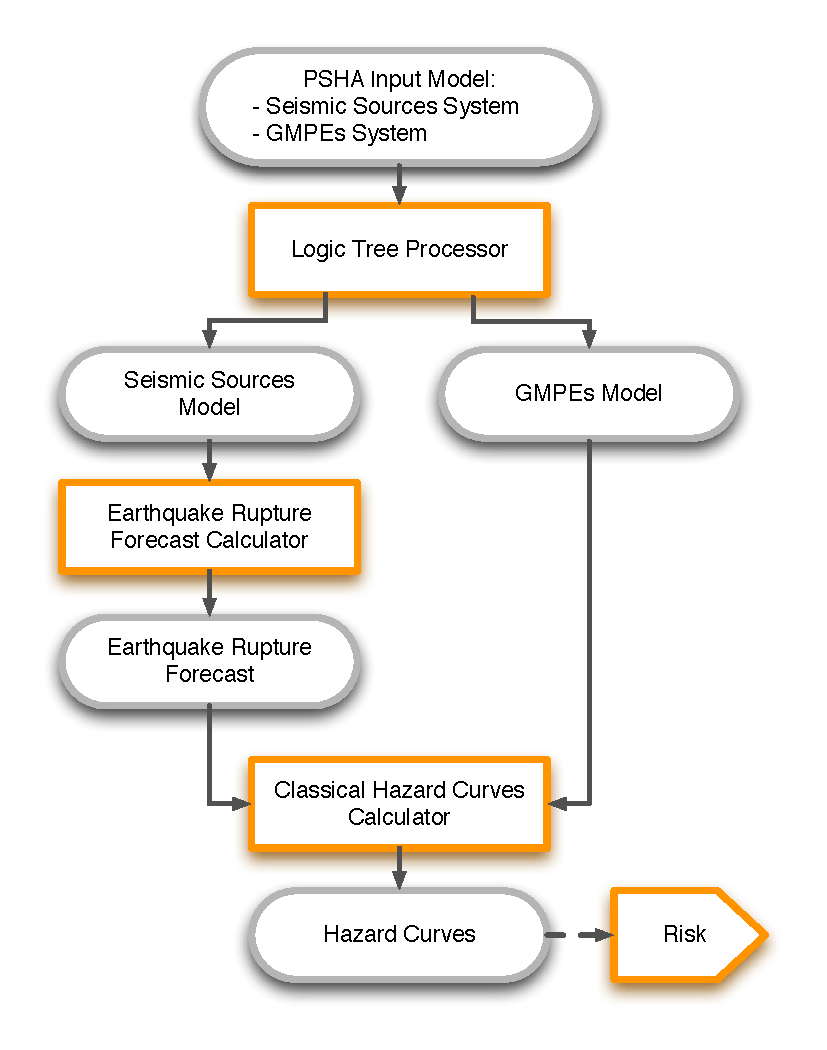
\includegraphics[width=12cm]{./Figures/Part_Hazard/classical_psha_workflow.eps}
\caption{Workflow for classical PSHA (boxes with purple border represent the 
calculators). Given a PSHA Input Model 
the Logic Tree Processor is responsible for creating a Seismic Sources model
and a ground motion model. 
The Seismic Sources model is then provided to the Earthquake Rupture Forecast 
calculator, which computes the ERF (the list of all earthquake ruptures in the 
source model with their probabilities of occurrence). 
Using the ERF and the GMPEs model the Classical PSHA calculator produces 
curves at the sites of interest.}
\label{classical_psha_workflow}
\end{center}
\end{figure}
% . . . . . . . . . . . . . . . . . . . . . . . . . . . . . . . . . . . < Figure
% ..............................................................................

As represented in Figure \ref{classical_psha_workflow}, the main calculators 
used to perform this analysis are:
\begin{enumerate}
%
\item \emph{Logic Tree Processor} \hfill \\
The Logic Tree Processor takes as an input the PSHA Input model. In case of 
the Seismic Sources, using the one of the Initial Seismic Sources Models and 
and by 'harvesting' the information contained in the Seismic Sources Logic Tree
- that is to sample the epistemic uncertainties - it creates a Seismic Sources 
Model (i.e. a model describing geometry and activity rates of each source 
without any epistemic uncertainty). 
%
Following the procedure just described the Logic Tree Processor creates a 
Ground Motion model (i.e. a data structure that associates to each tectonic 
region considered in the calculation a GMPE).
%
\item \emph{Earthquake Rupture Forecast Calculator} \hfill \\
The produced Seismic Sources Model is then used as input for the Earthquake 
Rupture Forecast (ERF) calculator which computes the probability of occurrence, 
over a specified time span, for each earthquake rupture produced by the source 
model.
\item \emph{Classical PSHA Calculator} \hfill \\
The cPSHA uses the ERF and the Ground Motion model to compute hazard curves on 
each site specified in the calculation settings.
\end{enumerate} 
%
%  - - - - - - - - - - - - - - - - - - - - - - - - - - - - - - - - - - - - - - -
\subsection{Event-Based Probabilistic Seismic Hazard Analysis}
\label{section:event-basedPSHA}
Input data for the Event-Based PSHA - as in the case of the Classical PSHA 
calculator - consist of a PSHA Input Model supplied to OQ together with a 
set of calculation settings.
%
% ..............................................................................
% . . . . . . . . . . . . . . . . . . . . . . . . . . . . . . . . . . . > Figure
\begin{figure}
\centering
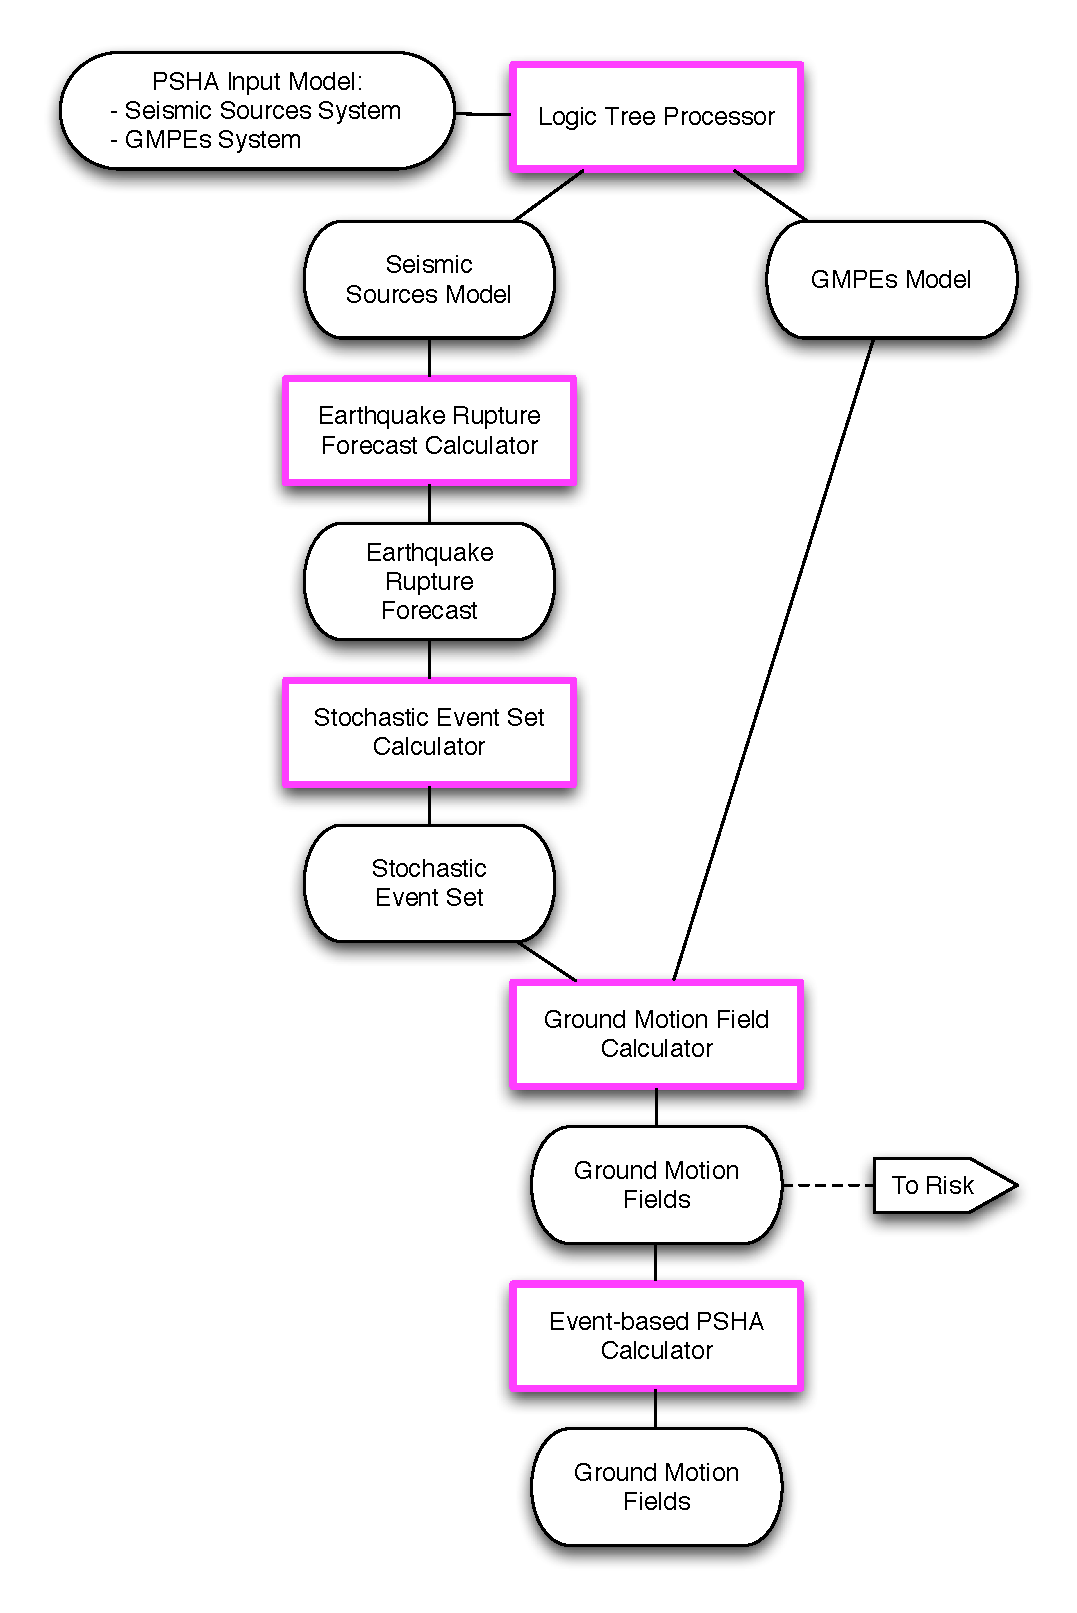
\includegraphics[width=12cm]{./Figures/Part_Hazard/event_based_workflow.eps}
\caption{Workflow for event-based PSHA. Similarly to the classical PSHA workflow 
(Figure \ref{classical_psha_workflow}), an ERF is computed, which is then used 
to generate a stochastic event set (representative of the seismic activity of 
a region in a given time span). Each event is then utilized to calculate a 
ground motion field over a region of interest.}
\label{event_based_workflow}
\end{figure}
% . . . . . . . . . . . . . . . . . . . . . . . . . . . . . . . . . . . < Figure
% ..............................................................................
As represented in Figure \ref{event_based_workflow}, the main calculators 
used to perform this analysis are:
\begin{enumerate}
%
\item \emph{Logic Tree Processor} \hfill \\
The Logic Tree Processor was already 
introduced in the description of the cPSHA workflow (see section 
\ref{section:classicalPSHA} at page \pageref{section:classicalPSHA}).
%
\item \emph{Earthquake Rupture Forecast Calculator} \hfill \\ 
The Logic Tree Processor was already 
introduced in the description of the cPSHA workflow (see section 
\ref{section:classicalPSHA} at page \pageref{section:classicalPSHA}).
%
\item \emph{Stochastic Event Set Calculator} \hfill \\
The Stochastic Event Set Calculator generates a Stochastic Event set 
by sampling each rupture contained in the ERF according to its 
probability of occurrence. Usually a Stochastic Event Set (SES) contains
a large number of seismicity history each one representative of a  
possible collection of events that can be produced by the seismic sources
considered in an analysis during the time span fixed for the calculation
of hazard (normally corresponding to 50 years).
%
\item \emph{Ground Motion Field Calculator} \hfill \\
The Ground Motion Field Calculator computes for each event contained in a 
Stochastic Event Set - provided as an input - a realization of the 
ground shaking taking into account the aleatory uncertainties in 
the ground motion model. Eventually, the Ground Motion Field calculator 
can consider the spatial correlation of the ground motion during the 
generation of the GMF.
%
\item \emph{Event-based PSHA Calculator} \hfill \\
The event-based PSHA calculator takes a (large) set of ground motion 
fields representative of the possible shaking that the investigated 
area can eventually experience over a (large) time span and for each 
grid node in a ground motion fields computes the corresponding hazard 
curve. 
%
This procedure is computationally intensive and is not recommended for 
investigating the hazard over large areas. 
\end{enumerate}

The Logic Tree Processor and the Earthquake rupture forecast were already 
introduced during the descrption of the cPSHA workflow (see section 
\ref{section:classicalPSHA} at page \pageref{section:classicalPSHA}).
%
%  - - - - - - - - - - - - - - - - - - - - - - - - - - - - - - - - - - - - - - -
\subsection{Deterministic Seismic Hazard Analysis}
\label{section:deterministicSHA}
% Deterministic
For deterministic SHA (DSHA), the input data consist of a single earthquake 
rupture model and a single ground motion model. Using the Ground Motion Field 
Calculator, multiple realizations of ground shaking can be computed, each 
realization sampling the aleatory uncertainties in the ground motion model.

As represented in Figure \ref{deterministic_workflow}, the main calculators 
used to perform this analysis are:
\begin{enumerate}
\item \emph{Ground Motion Field Calculator} \hfill \\
The Ground Motion Field Calculator was already 
introduced during the descrption of the ePSHA workflow (see section 
\ref{section:event-basedPSHA} at page \pageref{section:classicalPSHA}).
\end{enumerate}
% ..............................................................................
% . . . . . . . . . . . . . . . . . . . . . . . . . . . . . . . . . . . > Figure
\begin{figure}[!hb]
\centering
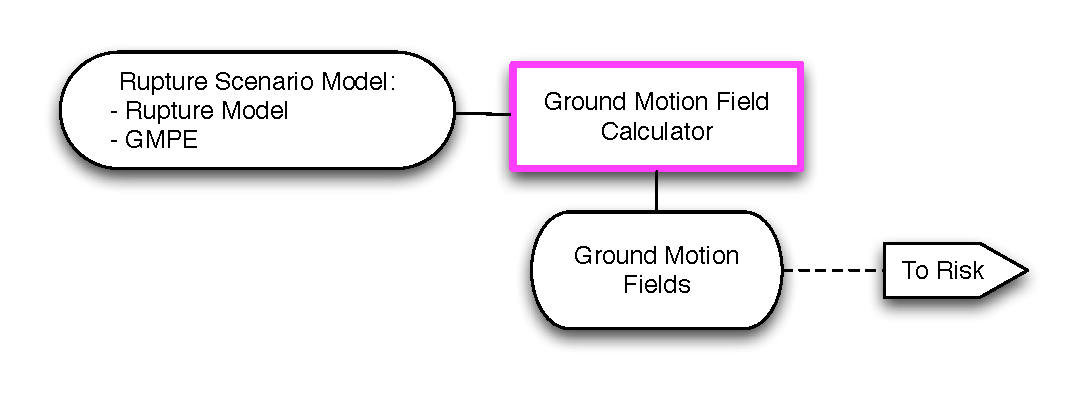
\includegraphics[width=12cm]{./Figures/Part_Hazard/deterministic_workflow.eps}
\caption{Workflow for deterministic SHA. Given a rupture scenario model, 
consisting of an earthquake rupture model, plus a GMPE, the ground motion 
field calculator can compute multiple ground motion field realizations (by 
taking into account GMPE aleatory uncertainties).}
\label{deterministic_workflow}
\end{figure}
% ..............................................................................
% . . . . . . . . . . . . . . . . . . . . . . . . . . . . . . . . . . . > Figure
%
% More details in the next chapters
%Next chapters discuss in more details the data model and the calculators. 
%Chapter \ref{chap:hazinp} describe the input data definition, that is the 
%different options for modeling seismogenic sources and how to include 
%epistemic uncertainties in both seismicity and ground motion models in 
%the form of a logic tree; Chapter \ref{chap:hazinp} also incorporates 
%the description of the logic tree structure adopted. 
%
%The methodology adopted to process the logic tree structure and the 
%definition and modeling of earthquake ruptures for the different 
%seismogenic source typologies are the topics of Chapter \ref{chap:erf}. 
%
%Chapter \ref{chap:hazcalc} describes the theoretical framework behind the main 
%hazard calculator available in OpenQuake: classical PSHA calculator and event 
%based calculator.
% ==============================================================================
% ------------------------------------------------------------------------------
% ------------------------------------------------------------------------- Part
\part{Appendixes}
\appendix
% ------------------------------------------------------------------------------
\chapter{Smoke Tests: Hazard}
	\input{./oqum_Part_Appendix/smokeTestHaz.tex}
% ------------------------------------------------------------------------------
\chapter{Smoke Tests: Risk}
	\input{./oqum_Part_Appendix/smokeTestRisk.tex}
% ==============================================================================
% ----------------------------------------------------------------- Bibliography
\bibliographystyle{apalike}
\bibliography{./Bibliography/hazard,./Bibliography/risk,./Bibliography/sei}
% ==============================================================================
% ------------------------------------------------------------------------ Index
\printglossaries
\printindex
\cleardoublepage
% Final empty page
\hfill \\ \thispagestyle{empty} \clearpage 
% ==============================================================================
% ------------------------------------------------------------------- Back Cover
\newgeometry{hmargin={0cm,-0.4cm},height=29.7cm}
\thispagestyle{empty}
\psset{unit=1cm}
\begin{pspicture}(0,0)(21cm,29.7cm)
	\psframe[fillstyle=solid,linecolor=gray02,fillcolor=white]
		(0.0cm,0.0cm)(21cm,15.0cm)
	\psframe[fillstyle=solid,linecolor=white,fillcolor=white]
		(0.0cm,15.0cm)(21cm,29.7cm)
	\psframe[fillstyle=solid,linecolor=orange01,fillcolor=orange01]
		(0.0cm,15.0cm)(21cm,15.5cm)
	\psframe[fillstyle=solid,linecolor=orange01,fillcolor=orange01]
		(0.0cm,25.0cm)(21cm,25.1cm)
\end{pspicture}
%
\end{document}
